%% Prepared for submission to Data & Knowledge Engineering (Elsevier).
%% Built on the official Elsevier elsarticle LaTeX authoring template
%% (elsarticle.cls, 2025/01/11 v3.4c) and the elsarticle-num.bst
%% numbered-reference bibliography style, per DKE's own submission guide
%% (single-anonymized review; double-column for LaTeX submissions).
%% All quantitative results below are computed from the frozen result
%% artifacts (see results/final_resubmission_method/ and the DKE stage-1
%% migration audit in docs/).

\documentclass[3p,times]{elsarticle}

\usepackage{graphicx}
\usepackage{multirow}
\usepackage{amsmath,amssymb,amsfonts}
\usepackage{booktabs}
\usepackage{tabularx}
\usepackage{algorithm}
\usepackage{algorithmicx}
\usepackage{algpseudocode}
\usepackage{url}
\usepackage{hyperref}

\journal{Data \& Knowledge Engineering}

\begin{document}

\begin{frontmatter}

\title{Retrieval-Assisted Instantiation of Natural-Language Optimization Problems}

\author[yingwu]{Soroush Vahidi\corref{cor1}\fnref{orcid}}
\ead{sv96@njit.edu}
\cortext[cor1]{Corresponding author.}
\fntext[orcid]{ORCID: 0000-0003-1934-6282.}
\affiliation[yingwu]{organization={Ying Wu College of Computing, New Jersey Institute of Technology}, addressline={University Heights}, city={Newark}, postcode={07102-1982}, state={NJ}, country={USA}}

\begin{abstract}
Many engineering optimization problems are first described in natural language and only later translated into formal mathematical models, but this translation remains difficult to automate reliably. Rather than targeting full solver-ready generation, this paper studies a narrower intermediate task: retrieval-assisted optimization problem instantiation, viewed as a knowledge-processing problem of grounding natural-language numeric evidence into a structured, typed optimization schema. The contribution is a transparent and reproducible framework that first retrieves the most compatible optimization schema from a fixed catalog and then deterministically instantiates that schema's scalar parameters from numeric evidence in the text, combining lexical schema retrieval, rule-based numeric extraction, coarse type inference, and deterministic compatibility-based slot assignment. We evaluate the framework on the NLP4LP benchmark of natural-language optimization problems, together with complementary structural and solver-backed validation subsets. Schema retrieval is already strong across query variants, with term frequency--inverse document frequency (TF--IDF) retrieval achieving the best average top-1 schema accuracy (Schema R@1 $=0.9094$ on original-text queries). The strongest non-oracle method reaches an InstantiationReady score of $0.8006$ ($0.7704$ under a stricter schema-gated criterion), while an oracle control with perfect schema retrieval reaches $0.8489$: this modest oracle gain shows that the main remaining bottleneck is downstream number-to-slot grounding rather than schema retrieval itself. A numeric-extraction ablation supports this conclusion. Restricted structural and solver-backed subset studies further suggest downstream optimization-oriented usefulness on compatible cases, without claiming benchmark-wide solver readiness.
\end{abstract}

\begin{keyword}
natural language processing \sep optimization modeling \sep knowledge representation \sep information retrieval \sep semantic grounding \sep intelligent information systems
\end{keyword}

\end{frontmatter}

\section{Introduction}

Many real-world engineering and operations problems are first described in natural language before they are formalized as optimization models. Analysts, planners, and domain experts specify resource limits, costs, capacities, proportions, and operational rules in text long before these elements are translated into a mathematical program. This gap between informal problem descriptions and formal optimization artifacts is a central concern of knowledge engineering: translating unstructured textual knowledge into a structured, machine-interpretable model requires both understanding the natural-language description and aligning it with an appropriate formal structure \cite{affolter2019nli,ramamonjison2022autoformulation,ramamonjison2023nl4opt}. A system that reliably connects a textual problem description to an appropriate optimization structure can reduce modeling effort, improve accessibility, and support practitioners during early stages of formalization.

This paper adopts a narrower but practically meaningful formulation: retrieval-assisted optimization-problem instantiation over a fixed catalog of structured optimization schemas. Rather than synthesizing an arbitrary mathematical program, the system first retrieves the most compatible optimization schema from a fixed catalog and then deterministically instantiates that schema's scalar parameters from numeric evidence in the text. This framing separates two issues that end-to-end systems often conflate: identifying the correct broad problem structure, and grounding the numerical content of the query into the correct scalar roles of that structure. Because eligible parameter slots are determined by the predicted schema, downstream performance remains retrieval-dependent by construction, which lets the experiments measure whether improved retrieval translates into better structured recovery. Viewing the catalog as a structured knowledge base and retrieval as knowledge-base selection, the task becomes an instance of knowledge-driven model instantiation, connecting directly to knowledge representation and information retrieval \cite{nlp4lp_dataset,ahmaditeshnizi2024optimus_icml,sheetrit2024rematch}.

Full translation from natural language to optimization models remains difficult for both families of existing approaches. Retrieval-based and lexical systems can select plausible candidate structures from text, but they do not by themselves recover the quantities needed to instantiate a model, and their lexical matching can be brittle under paraphrase. End-to-end large-language-model-based systems can generate formulations, solver code, or executable outputs from text \cite{ahmaditeshnizi2024optimus_icml,zhang2024optllm,ahmed2025opt2code}. However, they combine several sources of difficulty at once, making it hard to determine which intermediate capabilities are reliable, which stages contribute most to failure, and which parts of the pipeline provide practical value for engineering workflows \cite{astorga2025autoformulation,huang2025orlm,lu2025optmath}. These complementary limitations motivate studying an intermediate capability on its own.

In particular, a question that end-to-end settings obscure is where the main difficulty lies: is it in retrieving the correct broad optimization structure from a known catalog, or in grounding the numerical content of the query into the correct scalar roles once that structure has been identified? Answering this question requires a formulation in which the two stages can be evaluated separately and in which downstream performance remains conditioned on the retrieval decision. Such a decomposition is important not only for diagnostics but also for practice, because it determines where future effort in language-to-optimization pipelines should be invested.

To address this question, we study a fully deterministic and transparent pipeline. Given a natural-language query, the system ranks the fixed catalog of candidate schemas using standard lexical retrieval (BM25, TF--IDF, or latent semantic analysis), selects the top-ranked schema, and uses that schema to determine which scalar parameter slots are eligible. Numeric mentions are extracted from the query by rule-based methods, assigned a coarse type, and matched to eligible slots by a deterministic no-reuse compatibility procedure. Every intermediate decision -- which schema was selected, which slots were eligible, which mentions were extracted, and how assignments were made -- is inspectable and reproducible, providing the transparency required for human oversight in decision-support workflows \cite{biemans2025explainableoptimization,powell2025scheduling_explanations}.

We evaluate the framework on the \textsc{NLP4LP} benchmark of natural-language optimization problems \cite{nlp4lp_dataset,ahmaditeshnizi2024optimus_icml}, a curated collection of linear- and mixed-integer-programming descriptions. Schema retrieval is already strong across query variants, with TF--IDF achieving the best average top-1 schema accuracy (Schema R@1 $=0.9094$ on original-text queries). The strongest non-oracle method reaches an \textit{InstantiationReady} score of $0.8006$ ($0.7704$ under a stricter schema-gated criterion), while an oracle control with perfect schema retrieval reaches $0.8489$; this modest oracle gain, corroborated by a numeric-extraction ablation, shows that the main remaining bottleneck is downstream number-to-slot grounding rather than schema retrieval itself. Restricted structural and solver-backed subset studies further suggest downstream optimization-oriented usefulness on compatible cases, without claiming benchmark-wide solver readiness.

This paper makes four contributions.
\label{subsec:intro_contributions}
First, it contributes a \emph{problem formulation and evaluation framework} that decomposes natural-language optimization understanding into two explicit, separately measurable stages -- schema retrieval and schema-conditioned scalar parameter grounding -- connected by a retrieval-dependent evaluation design in which eligible parameter slots are determined by the predicted schema rather than the gold schema. Second, it contributes a \emph{deterministic, inference-time LLM-free methodology}: a fully deterministic pipeline that maps numeric textual evidence to typed optimization-schema parameters through lexical schema retrieval, rule-based numeric extraction, coarse type inference, and no-reuse compatibility-based slot assignment, with every intermediate decision inspectable and reproducible, and without invoking any large language model at inference time. Third, it contributes a \emph{comprehensive empirical diagnosis} of where this pipeline succeeds and fails, combining oracle controls, a strict-metric sensitivity analysis, a numeric-extraction ablation, paired bootstrap significance tests, lexical-overlap robustness tests, and an error taxonomy; together these consistently identify semantic quantity-to-role grounding -- not schema retrieval -- as the dominant bottleneck. Fourth, it contributes \emph{reproducibility and downstream validation}: a public implementation together with restricted structural and solver-backed evidence computed from frozen artifacts, providing measurable evidence of downstream optimization-oriented usefulness on compatible cases.

The remainder of the paper is organized as follows. Section~\ref{sec:related_work} reviews related work. Section~\ref{sec:method} presents the problem formulation, retrieval stage, deterministic parameter-instantiation backbone, and evaluation-oriented design choices. Section~\ref{sec:experiments} describes the experimental setup and reports retrieval performance, downstream utility, structural and solver-backed validation, and error analysis. Section~\ref{sec:conclusion} concludes with the main findings, limitations, and directions for future work.

\section{Related Work}
\label{sec:related_work}

\subsection{Natural Language and Mathematical Optimization Modeling}
\label{subsec:rw_nl_modeling}

An important early direction has focused on helping users convert textual problem descriptions into formal optimization artifacts. Ramamonjison et al.\ introduced an assistive auto-formulation framework in which natural-language problem descriptions are mapped to editable optimization-model suggestions, combining automatic support with interactive modeling assistance \cite{ramamonjison2022autoformulation}. This line of work also led to benchmark-oriented efforts such as \textsc{NL4Opt}, which helped establish natural-language-to-optimization as a shared evaluation problem and emphasized the extraction of optimization entities and machine-interpretable structure from text \cite{ramamonjison2023nl4opt}. Related work such as \textsc{LaTeX2Solver} explored hierarchical parsing pipelines for converting semi-structured mathematical documents into optimization-oriented code representations \cite{ramamonjison2023latex2solver}. Beyond full model generation, \textsc{Ner4Opt} frames optimization modeling support as an information-extraction problem over natural-language descriptions, focusing on optimization-relevant entities and quantities needed for downstream modeling \cite{kadioglu2024ner4opt}. Recent benchmark work has broadened the scope beyond linear and mixed-integer programming: \textsc{Text2Zinc} introduces a cross-domain dataset for optimization and satisfaction problems in \textsc{MiniZinc}, while \textsc{CP-Bench} evaluates large language models for constraint modeling across multiple constraint-programming systems \cite{singirikonda2025text2zinc,michailidis2025cpbench}. Related work such as \textsc{EHOP} further shows that the linguistic presentation of optimization-style tasks can materially affect model performance \cite{duchnowski2025ehop}. At a broader level, recent surveys document the rapidly growing interaction between large language models and optimization \cite{huang2024llmoptimization,huang2025llmsmathmodeling,xiao2025optmodelingsurvey}.

\subsection{LLM-Based Optimization-Model Generation}
\label{subsec:rw_llm_generation}

A second and increasingly prominent direction uses large language models for end-to-end optimization modeling, producing formulations, solver code, or executable outputs. \textsc{OptiMUS} studies how large language models, together with solver feedback, can formulate, implement, debug, and solve linear and mixed-integer programming problems from natural-language descriptions, evaluated on the \textsc{NLP4LP} benchmark \cite{ahmaditeshnizi2024optimus_icml,ahmaditeshnizi2024optimus03}. OptLLM proposes an LLM-centered framework augmented with external solvers for converting natural-language optimization requests into formulations, code, and solutions \cite{zhang2024optllm}. \textsc{Chain-of-Experts} coordinates a set of role-specialized LLM agents under a conductor that revises the formulation through forward construction and backward reflection \cite{xiao2024chainofexperts}. \textsc{LLMOPT} instead fine-tunes a model end-to-end on a five-element optimization formulation together with automated model classification and solver-code generation \cite{jiang2025llmopt}. More recently, retrieval-augmented generation has been explored in this setting: \textsc{OPT2CODE} combines retrieval, code generation, and judge-based checking to translate linear-programming descriptions into solver-executable code \cite{ahmed2025opt2code}, and \textsc{Autoformulation} frames the task as a search over hierarchically decomposed formulation components, combining Monte-Carlo tree search with LLM-based hypothesis generation and symbolic pruning \cite{astorga2025autoformulation}. Question-partitioning strategies have been shown to help LLMs structure the modeling process \cite{pan2025pamop}. Beyond prompting- and generation-oriented systems, recent work develops reusable training pipelines and synthesis frameworks: \textsc{ORLM} contributes a customizable framework for training large models on optimization-modeling tasks with solver-guided feedback \cite{huang2025orlm}, \textsc{OptMATH} introduces a scalable bidirectional data-synthesis framework that expands optimization-modeling training corpora \cite{lu2025optmath}, and \textsc{ReSocratic} synthesizes optimization demonstrations in reverse for supervised fine-tuning, together with the \textsc{OptiBench} benchmark \cite{yang2025optibench}. Evaluation-oriented benchmarks in the operations-research domain include \textsc{ORQA}, a multiple-choice benchmark probing LLM reasoning about optimization models \cite{mostajabdaveh2025orqa}, and \textsc{Mamo}, a solver-backed modeling benchmark \cite{huang2025llmsmathmodeling}. Finally, very recent work applies reinforcement learning and foundation-model training to modeling and solving: \textsc{OR-R1} automates modeling and solving via test-time reinforcement learning \cite{ding2026orr1}, and \textsc{DeepOR} trains a deep-reasoning foundation model for optimization modeling \cite{xiao2026deepor}.

\subsection{Retrieval, Schema Selection, and Structured Grounding}
\label{subsec:rw_retrieval}

The proposed pipeline builds on standard lexical retrieval and is closely related to work on schema selection and structured grounding in data and knowledge engineering. BM25 \cite{robertson2009bm25}, TF--IDF cosine retrieval \cite{pedregosa2011sklearn}, and latent semantic analysis \cite{deerwester1990lsa} provide the deterministic ranking backbones evaluated in this paper. The broader problem of connecting natural language to structured data has a long tradition: \textsc{Spider} established a large-scale, cross-domain text-to-SQL benchmark requiring generalization to new database schemas \cite{yu2018spider}, and comparative surveys analyze natural-language interfaces for databases and the translation of questions into formal query languages \cite{affolter2019nli}. Closer to the present setting, schema matching -- aligning elements of a source schema with those of a target schema -- has recently been combined with retrieval and LLMs in \textsc{ReMatch} \cite{sheetrit2024rematch}. Within the DKE community, LLMs have been used to support conceptual design of multidimensional cubes \cite{rizzi2025conceptual} and to act as an intermediate semantic layer for query answering over heterogeneous data \cite{atzeni2026semantic}. These works share with ours a concern for grounding natural-language evidence into structured, typed artifacts, but they target relational or multidimensional schemas rather than optimization-model templates.

\subsection{Position of the Present Work}
\label{subsec:rw_position}

Our work is most closely related to natural-language-to-optimization modeling, but it occupies a different point in the design space from both end-to-end generation systems and component-level extraction systems. End-to-end systems aim to produce complete formulations, solver code, or solver-ready models \cite{ahmaditeshnizi2024optimus_icml,zhang2024optllm,ahmed2025opt2code,astorga2025autoformulation}; we instead focus on a narrower intermediate task -- retrieval-assisted schema grounding followed by scalar parameter instantiation. Component-level extraction approaches such as \textsc{Ner4Opt} recover entities and quantities \cite{kadioglu2024ner4opt}; we go further by making downstream slot eligibility depend explicitly on the retrieved schema, so that downstream evaluation remains structurally tied to schema-selection quality. This design isolates an empirically important question that is often obscured in end-to-end pipelines: whether the main difficulty lies in retrieving the correct broad optimization structure or in grounding the numerical content of the query into the correct scalar roles once that structure has been identified. The framework is fully deterministic and transparent, which makes it possible to analyze where gains arise and where residual errors remain. In contrast to end-to-end LLM systems, which require generative inference (typically through paid APIs or dedicated GPU compute) to produce a formulation or program, the proposed method requires no large language model at inference time and no learned retriever or extractor. This is not a claim that lexical, deterministic grounding is generally superior to LLM-based modeling; rather, the two approaches address different points on a cost--capability tradeoff. LLM systems target broader, open-ended synthesis of complete models, whereas the present system targets fixed-catalog schema instantiation with fully inspectable intermediate decisions. We therefore position this paper as a study of retrieval-assisted optimization-model support: not full natural-language-to-optimization compilation, but schema retrieval and schema-conditioned scalar instantiation as measurable and practically useful components of a broader engineering decision-support workflow.

\section{Methodology}
\label{sec:method}

\subsection{Problem Formulation}
\label{subsec:method_problem}

We study a retrieval-assisted instantiation task for natural-language optimization descriptions. Given a query that describes an optimization problem, the objective is not to generate a complete mathematical program directly. Instead, the system produces two structured outputs: (i) a schema prediction that identifies the most compatible optimization template from a fixed catalog, and (ii) scalar parameter assignments for the retrieved schema. This formulation captures an important intermediate step in natural-language-to-optimization pipelines: before a full model can be constructed, the system must identify an appropriate template and recover the key quantities needed to instantiate it \cite{nlp4lp_dataset,ramamonjison2023nl4opt,ahmaditeshnizi2024optimus_icml}.

We cast the task as a two-stage decision process. In the first stage, the system performs \emph{schema retrieval}: given a query $q$, it ranks a catalog $\mathcal{S}=\{s_1,\dots,s_M\}$ of candidate optimization schemas and returns the top-ranked schema
\begin{equation}
\hat{s}=\arg\max_{s \in \mathcal{S}} \mathrm{score}(q,s).
\label{eq:top1_schema}
\end{equation}
Each schema represents an optimization template together with its associated parameter structure. In the second stage, the system performs \emph{parameter instantiation}: conditioned on the retrieved schema $\hat{s}$, it extracts numeric mentions from the query and assigns them to the scalar parameter slots specified by $\hat{s}$ using deterministic grounding rules. The second stage is explicitly retrieval-dependent: if schema retrieval is incorrect, the set of eligible parameter slots may also be incorrect, reducing downstream coverage and readiness even when the query still contains informative numeric evidence.

In this paper, the term \emph{schema} refers to the retrieved optimization template together with the scalar parameter structure to be instantiated. The resulting task is narrower than full natural-language-to-optimization translation. The main benchmarked setting does not attempt to synthesize a complete optimization model, recover all variables and constraints, or reconstruct structured parameter objects such as lists, vectors, or dictionaries. Rather, the focus is on whether schema retrieval can anchor a natural-language description to a plausible optimization template, and whether deterministic grounding can recover useful scalar values once that template has been selected.

Our scope is intentionally restricted in three ways. First, benchmark-level downstream evaluation is limited to scalar numeric parameters. Second, the core retrieval-and-grounding pipeline is fully deterministic and uses no large language model, no learned retriever, and no learned extractor. Third, the main benchmark study evaluates schema-conditioned scalar recovery rather than full end-to-end model generation. These restrictions are deliberate: they isolate an interpretable intermediate capability and allow precise analysis of where performance gains and failures arise. At the same time, the broader experimental section complements this benchmarked formulation with structural and solver-backed subset validation, including structural-validity analysis and a restricted solver-backed study on compatible instances. These additional experiments are intended to assess downstream practical relevance, not to redefine the core task studied here.

Formally, let $G(q)$ denote the set of scalar gold parameters associated with query $q$, and let $P(\hat{s})$ denote the scalar parameter keys exposed by the retrieved schema $\hat{s}$. The downstream evaluator considers only the eligible slot set
\begin{equation}
E(q,\hat{s}) = G(q) \cap P(\hat{s}),
\label{eq:eligible_slots}
\end{equation}
that is, the scalar gold parameters whose keys are present in the predicted schema. This choice makes downstream evaluation retrieval-dependent by construction. Even when a query contains the correct numeric evidence, an incorrect schema can reduce structural overlap and therefore lower downstream performance. The formulation is designed to measure not only whether the correct schema is retrieved, but also whether improved schema retrieval yields measurable gains in structured parameter instantiation.

Retrieval quality is measured by whether the top-ranked schema matches the gold schema, while downstream quality is measured by how well scalar slots from the retrieved schema can be instantiated from the query text. As the experiments later show, retrieval on \textsc{NLP4LP} is already strong, whereas the main remaining difficulty lies in grounding extracted numbers to the correct scalar roles within the chosen schema. The formulation adopted here therefore isolates the stage that currently matters most empirically: deterministic number-to-slot grounding after schema retrieval.

\subsection{Retrieval-Based Schema Identification}
\label{subsec:method_retrieval}

The first stage of the framework performs \emph{schema identification by retrieval}. Given a natural-language optimization description, the system selects the most compatible candidate from a fixed catalog of benchmark-induced schema documents. We formulate this stage as a ranking problem over a finite candidate set $\mathcal{S}$. Each candidate document is indexed by a schema identifier and paired with the textual schema description used by the evaluation pipeline. Given an input query, the retriever scores the query against every candidate document and returns a ranked list. In the present pipeline, only the highest-ranked candidate is used, so retrieval is treated as a top-1 schema selection problem rather than a shortlist-generation or interactive retrieval task.

It is important to clarify what a ``schema candidate'' means in this setting. The retrieval corpus is the benchmark-induced catalog used by the evaluation pipeline, which contains 335 candidate schema documents. Thus, the retrieval task in this paper is neither open-domain optimization search nor coarse classification into a small number of broad problem families. Instead, it is a fixed-catalog identification problem: for each query, the system must select the single benchmark schema document that serves as the structural template for downstream grounding. This benchmark-specific formulation is deliberate because the goal of the paper is to study whether natural-language optimization descriptions can first be anchored to a usable template and then instantiated deterministically.

Operationally, the retrieved schema serves as the structural anchor for downstream instantiation. Through its identifier, the system accesses the associated parameter structure and uses that structure to determine which scalar slots are eligible for filling. The retrieval stage therefore does \emph{not} attempt to reconstruct a full symbolic optimization model, derive solver-ready constraints, or generate variables and objectives directly. Instead, it selects the most plausible template index from which the downstream stage can obtain an expected set of scalar parameter roles \cite{nlp4lp_dataset,ramamonjison2023nl4opt,ahmaditeshnizi2024optimus_icml}.

This fixed-catalog setup should also be distinguished from label-only classification. The retriever does not predict an abstract class name from a small closed set of manually engineered categories. Rather, it ranks textual schema documents using their natural-language content. This distinction matters because the empirical question in our benchmark is not merely whether a query belongs to a broad optimization family, but whether it can be aligned to the \emph{specific} schema document whose parameter inventory is then used for downstream slot grounding. Retrieval quality therefore directly affects the structural conditions under which the second stage operates.

We evaluate three deterministic lexical retrieval baselines: BM25 \cite{robertson2009bm25}, TF--IDF cosine retrieval \cite{pedregosa2011sklearn}, and latent semantic analysis (LSA) \cite{deerwester1990lsa}. All three retrievers are deterministic, CPU-based, and operate directly on schema-catalog text without benchmark-specific training, dense neural encoders, or learned reranking. Table~\ref{tab:retrieval_backbones} summarizes their roles in the pipeline.

For a query $q$, each retriever produces a score for every candidate schema $s \in \mathcal{S}$, and the predicted schema is
\begin{equation}
\hat{s}(q) = \arg\max_{s \in \mathcal{S}} \mathrm{score}(q,s).
\label{eq:schema_retrieval}
\end{equation}
Only $\hat{s}(q)$ is passed to the downstream instantiation stage. This top-1 design matches the evaluation goal of the paper: we ask whether the system can identify a single usable schema that supports deterministic slot filling, rather than whether it can produce a longer candidate list for later interaction or reranking.

To interpret retrieval performance, we use two diagnostic references in the broader pipeline. The first is an \emph{oracle} control, which replaces the retrieval output with the gold schema identifier and therefore exposes downstream behavior under perfect schema selection. The second is a \emph{random} reference. For retrieval-only evaluation, this random reference is the theoretical top-1 chance rate under uniform selection over the 335 candidate schema documents, namely $1/335 \approx 0.0030$. For downstream evaluation, ``random'' instead denotes a uniformly chosen schema passed through the same deterministic instantiation pipeline. These references are included only to calibrate interpretation; they are not competing learned retrievers.

Because the retrieved schema determines the candidate slot inventory used downstream, retrieval errors propagate structurally. If the wrong schema is selected, the second stage may inherit a slot set that only partially overlaps the gold instance or that mismatches the intended scalar roles altogether. This can reduce downstream coverage, type agreement, and per-query readiness even when the query still contains relevant numeric evidence. Conversely, strong retrieval creates more favorable structural conditions for deterministic grounding by supplying a more appropriate set of candidate slots.

This formulation emphasizes retrieval as \emph{schema grounding} rather than full optimization-model reconstruction: the first stage maps a free-form optimization description to a single candidate template whose scalar parameter structure can then be instantiated transparently. Retrieval is an important enabling step in the pipeline, but, as the experiments show, not the dominant empirical bottleneck.

\begin{table}[t]
\centering
\caption{Deterministic retrieval backbones used for schema identification.}
\label{tab:retrieval_backbones}
\small
\begin{tabularx}{\linewidth}{l l X}
\toprule
Method & Representation & Role in pipeline \\
\midrule
BM25 & Probabilistic lexical weighting & Sparse lexical baseline \\
TF--IDF & Weighted bag-of-words cosine similarity & Main deterministic retrieval backbone \\
LSA & Latent projection of TF--IDF features & Lower-dimensional lexical-semantic baseline \\
\bottomrule
\end{tabularx}
\end{table}

\subsection{Deterministic Parameter Instantiation}
\label{subsec:method_instantiation}

Given a natural-language query and a predicted schema, the second stage of the framework instantiates scalar parameter slots from textual numeric evidence. The output of this stage is a set of slot--value assignments associated with the retrieved schema. In the main benchmarked setting, this stage does not generate a complete optimization model and does not recover variables, constraints, or structured parameter objects. Its purpose is narrower: to recover scalar values that can be aligned with the parameter structure of the retrieved template.

The instantiation stage begins by extracting candidate numeric mentions from the query text using a fixed rule-based pattern matcher. The extractor recognizes integers, decimals, percentage expressions, currency-like forms, and comma-separated magnitudes. In degraded query settings, masked placeholders are preserved as special tokens but treated as numerically unknown, so they cannot support exact value recovery. Each extracted mention is then assigned a coarse type label from four buckets: \emph{percent}, \emph{integer}, \emph{currency}, and \emph{float}. Mention typing relies on deterministic surface cues such as percentage markers, currency markers, integer-valued forms, and local lexical context.

The predicted schema determines which parameter slots are eligible for instantiation. Operationally, the system obtains the parameter keys associated with the retrieved template and then restricts attention to scalar-valued slots. This restriction is deliberate. List-valued and dictionary-valued parameters correspond to more structured objects whose recovery would require additional representational assumptions, so the present framework focuses on scalar numeric instantiation. The instantiation problem is therefore defined over a finite set of eligible scalar slots together with a pool of extracted numeric candidates.

For each eligible slot, an expected type is inferred from its parameter name using deterministic rules. Parameters whose names indicate rates or fractions are mapped to \emph{percent}; names indicating counts or cardinalities are mapped to \emph{integer}; names suggesting monetary quantities are mapped to \emph{currency}; and all remaining scalar slots are mapped to \emph{float}. This shared typed representation places slots and extracted numeric mentions in a common compatibility space before assignment.

The simplest assignment rule used in the framework is typed greedy matching. Let $\mathcal{P}=\{p_1,\dots,p_m\}$ denote the eligible scalar slots induced by the predicted schema, and let $\mathcal{T}=\{t_1,\dots,t_n\}$ denote the extracted numeric mentions. In the typed-greedy setting, the selected mention for slot $p_i$ is the highest-scoring unused candidate under a deterministic compatibility rule,
\begin{equation}
t_i^{*} = \arg\max_{t \in \mathcal{T}\setminus \mathcal{U}_{i-1}} \mathrm{compat}(p_i,t),
\label{eq:typed_assignment}
\end{equation}
where $\mathcal{U}_{i-1}$ is the set of mentions already assigned in previous steps. The compatibility function prioritizes agreement between the expected slot type and the inferred mention type, together with deterministic tie-breaking based on local cues and extraction order. Once a mention is assigned, it is removed from the candidate pool and cannot be reused for later slots. This yields a one-pass deterministic assignment rule rather than a global combinatorial optimizer.

The broader method family evaluated in the paper extends this same backbone. In addition to lexical typed-greedy baselines, we consider deterministic grounding variants that modify how slot--mention compatibility is scored or revised after an initial assignment. These include constrained matching, semantic repair, optimization-role repair, acceptance reranking, and hierarchical acceptance reranking. Although these methods differ in scoring or repair strategy, they share the same core structure: deterministic numeric extraction, schema-conditioned scalar slot selection, coarse type inference, and no-reuse slot filling. This common backbone is summarized in Algorithm~\ref{alg:instantiation} and illustrated in Figure~\ref{fig:instantiation-pipeline}.

We use \emph{optimization-role compatibility} to refer to a deterministic, lexicon-based refinement of the basic type-compatibility signal used by \texttt{tfidf\_optimization\_role\_repair}. Beyond the coarse type label (\emph{percent}, \emph{integer}, \emph{currency}, \emph{float}), each slot name and its local query context are matched against a fixed lexicon of optimization-role cue words (e.g., terms indicating a capacity limit, a cost coefficient, a cardinality bound, or a derived count). When a candidate mention's local context shares a role cue with the slot, the deterministic assignment score in Eq.~\eqref{eq:typed_assignment} receives an additive bonus; when the mention's inferred type is incompatible with the slot's expected type, it receives a penalty large enough to make the mention non-preferred (though not strictly inadmissible, since ties and missing alternatives can still cause an incompatible mention to be assigned). We use \emph{admissibility} in this paper only in this graded, score-based sense -- a slot--mention pairing is more or less preferred under the compatibility rule -- rather than as a hard combinatorial constraint verified against a formal model of the optimization problem; the framework does not currently guarantee that an admissible-by-type assignment is also feasible or optimal for the underlying (unobserved) mathematical program. This is a heuristic, rule-based layer, and we report it as such: it is designed to break ties among type-compatible candidates using domain-typical lexical cues, not to provide a formal correctness guarantee.

To isolate the effect of type-aware matching, we also evaluate a \emph{numeric-extraction ablation} that corrects multiplicative ratio-word numeric expressions (e.g., ``twice'', ``double'', ``triple'') so that extracted values are scaled deterministically. As the experiments later show, this correction materially improves \textit{TypeMatch} and \textit{InstantiationReady} while leaving retrieval-dependent quantities much less changed, confirming that the main downstream gains arise from improved number-to-slot grounding rather than from changes in retrieval or mention extraction. We explain the correction only once here and refer to the comparison throughout as the numeric-extraction ablation.

In short, the instantiation stage is intentionally simple: numeric evidence is extracted from the query, typed using deterministic cues, filtered through the scalar parameter structure of the predicted schema, and assigned to slots by a deterministic no-reuse procedure. The resulting slot--value mapping is then evaluated downstream. In the broader paper, this benchmarked scalar-instantiation stage is complemented by restricted downstream validation on subsets, but the core methodology here remains a deterministic, schema-conditioned scalar grounding pipeline.

\begin{algorithm}[t]
\caption{Deterministic parameter instantiation pipeline. Numeric mentions are extracted from the query and typed using surface cues. In parallel, the predicted schema provides the eligible scalar slots, whose expected types are inferred from slot names. A deterministic compatibility-based assignment procedure then maps numeric mentions to slots without token reuse. Downstream variants differ in how slot--mention compatibility is scored or repaired.}
\label{alg:instantiation}
\small
\begin{algorithmic}[1]
\Require Query text $q$, predicted schema $\hat{s}$
\Ensure Slot--value mapping $A$
\State Extract numeric mentions $\mathcal{T}$ from $q$
\State Infer a coarse type for each mention in $\mathcal{T}$
\State Obtain parameter keys from schema $\hat{s}$
\State Restrict to eligible scalar slots $\mathcal{P}=\{p_1,\dots,p_m\}$
\State Infer an expected type for each slot in $\mathcal{P}$
\State Initialize assignments $A \leftarrow \emptyset$ and used-mention set $\mathcal{U}\leftarrow \emptyset$
\For{each slot $p_i \in \mathcal{P}$}
    \State Define candidate set $\mathcal{C}_i \leftarrow \mathcal{T} \setminus \mathcal{U}$
    \If{$\mathcal{C}_i = \emptyset$}
        \State \textbf{continue}
    \EndIf
    \State Score mentions in $\mathcal{C}_i$ using a deterministic slot--mention compatibility rule
    \State Select the highest-ranked mention $t_i^{*}$
    \State Assign $A[p_i] \leftarrow \mathrm{value}(t_i^{*})$
    \State Update $\mathcal{U} \leftarrow \mathcal{U} \cup \{t_i^{*}\}$
\EndFor
\State \Return $A$
\end{algorithmic}
\end{algorithm}

\begin{figure}[t]
  \centering
  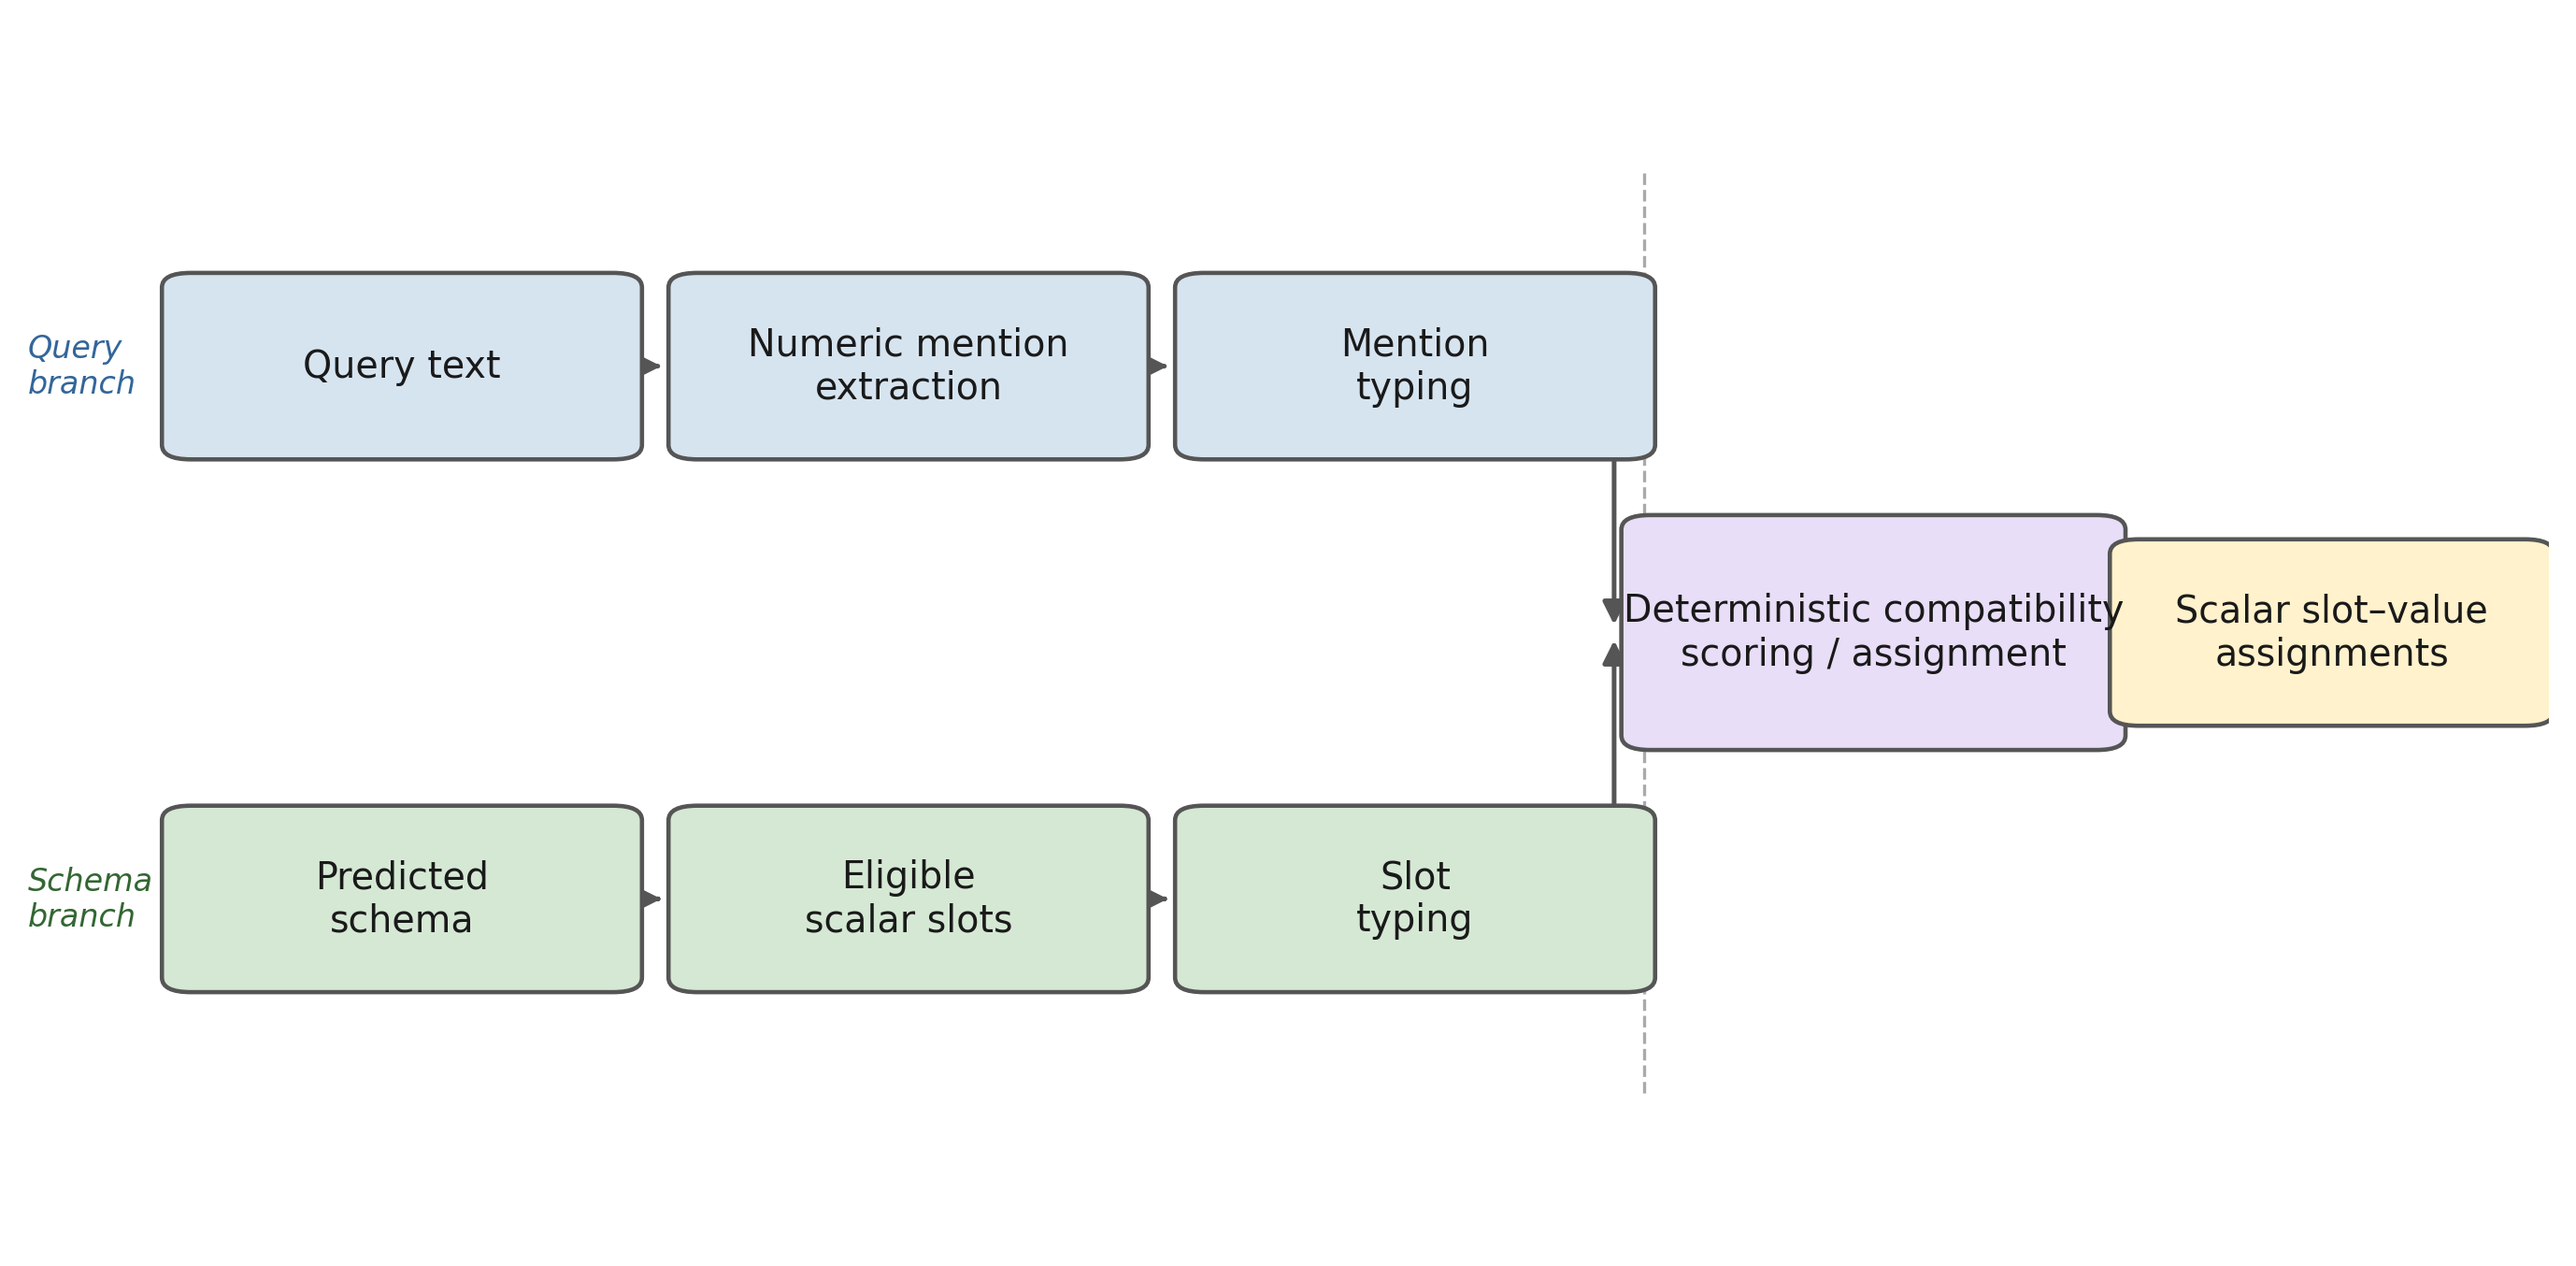
\includegraphics[width=0.82\linewidth]{figures/nlp4lp_instantiation_pipeline_v2.png}
  \caption{Schema-conditioned deterministic parameter instantiation. Numeric mentions are extracted from the query, typed using surface cues, filtered through the scalar slot inventory of the predicted schema, and assigned by a no-reuse compatibility rule. Downstream variants differ mainly in how slot--mention compatibility is scored or repaired.}
  \label{fig:instantiation-pipeline}
\end{figure}

\subsection{Evaluation-Oriented Design Choices}
\label{subsec:method_design}

The methodology is intentionally designed so that downstream evaluation remains sensitive to schema retrieval quality. In particular, the set of parameter slots eligible for instantiation is determined from the \emph{predicted} schema rather than from the gold schema. This choice is central to the formulation. If eligible slots were defined directly from the gold record, downstream coverage and readiness would no longer reflect schema-selection quality, and the evaluation would partially decouple retrieval from instantiation. By conditioning slot eligibility on the retrieved template, the framework ensures that retrieval errors propagate naturally into downstream performance through reduced structural overlap, lower slot availability, and weaker query-level readiness. At the same time, the evaluation avoids leakage: gold information is used for scoring, not for determining which schema is instantiated at inference time.

A second design choice restricts the main benchmarked downstream evaluation to scalar numeric parameters, which provide a common and reproducible substrate for comparing retrieval-conditioned instantiation across heterogeneous templates while avoiding the additional alignment and dimensionality assumptions required to reconstruct list- or dictionary-valued objects (Section~\ref{subsec:method_problem}).

As introduced in Section~\ref{subsec:method_retrieval}, the oracle and random references serve the same interpretive purpose throughout the paper. We refer to the oracle condition as an \emph{oracle control} (or oracle reference) rather than a formal upper bound: because \textit{InstantiationReady} depends on per-query type-inference and slot-eligibility details that are not guaranteed to be monotonic in schema correctness, the oracle condition is not mathematically certain to dominate every non-oracle method on every metric or subset, and Section~\ref{subsec:exp_engineering} reports a concrete case (the 20-instance solver-backed subset) where it does not.

The core study is intentionally solver-free and fully deterministic: no feasibility test, optimization run, or objective-level verification enters the core metrics, and the pipeline uses no large language model, learned retriever, or learned extractor. This keeps the central evaluation transparent and reproducible and lets the experiments answer a focused question -- how much structured instantiation utility deterministic retrieval and rule-based grounding can provide -- while downstream executability is examined separately on the restricted subsets of Section~\ref{subsec:exp_engineering}.

These choices also determine how the metrics should be read. \textit{InstantiationReady} is a diagnostic readiness criterion based on coverage and type consistency, not a guarantee of model correctness or solver compatibility; strong schema retrieval is not full optimization-model recovery; and successful scalar assignment is not feasibility- or optimality-verified instantiation. The framework is best viewed as a retrieval-assisted deterministic instantiation system that quantifies how schema grounding affects structured parameter recovery, with the restricted subset analyses addressing the separate question of downstream executable behavior on compatible cases.

\noindent\textbf{Note on generative-AI assistance.} The retrieval-and-grounding pipeline studied in this paper is itself fully deterministic and uses no large language model, learned retriever, or learned extractor (see above). Separately, during preparation of this work the author used ChatGPT and Gemini to assist with aspects of manuscript writing and used Cursor and GitHub Copilot to assist with coding; the author reviewed, verified, and edited all generated content and takes full responsibility for the content of the publication. No generative-AI tool is listed as an author, consistent with Elsevier's authorship policy.

\section{Experiments}
\label{sec:experiments}

\subsection{Experimental Setup}
\label{subsec:exp_setup}

We evaluate the proposed retrieval-assisted instantiation pipeline on the \textsc{NLP4LP} benchmark \cite{nlp4lp_dataset,ahmaditeshnizi2024optimus_icml}, a curated collection of linear- and mixed-integer-programming problem descriptions in which each instance pairs a natural-language description with a gold parameter record, a reference solver implementation, and, where available, a reference solution. Unless otherwise stated, the main benchmark results are measured on the benchmark test split, which contains 331 query instances. Each test query has exactly one gold optimization schema. Each test query is ranked against the benchmark-induced schema catalog used by the evaluation pipeline, which contains 335 candidate schema documents. Accordingly, retrieval is a 335-way top-1 identification task, and the corresponding random top-1 reference is the theoretical chance rate under uniform selection over this catalog, namely $1/335 \approx 0.0030$.

To assess robustness to surface degradation and reduced context, we evaluate three benchmark query variants. The \emph{orig} variant uses the original problem descriptions. The \emph{noisy} variant applies controlled lexical corruption, including lowercasing, token deletion, stopword reduction, and masking of some numeric expressions. The \emph{short} variant retains only the first sentence of each description. These variants allow us to test the same retrieval-and-grounding pipeline under full context, degraded wording, and substantially reduced context.

The retrieval stage ranks candidate schemas using only schema-catalog text. In the final reported benchmark comparison, we evaluate three deterministic lexical retrieval baselines: BM25 \cite{robertson2009bm25}, TF--IDF cosine retrieval implemented with \textsc{scikit-learn} \cite{pedregosa2011sklearn}, and latent semantic analysis (LSA), obtained by applying truncated singular value decomposition to TF--IDF vectors \cite{deerwester1990lsa}. In all downstream experiments, only the top-ranked schema is passed to the instantiation stage. We also report an \emph{oracle} control in which the retrieved schema is replaced by the gold schema, thereby isolating downstream grounding difficulty from retrieval error.

Given a query and a predicted schema, the downstream stage instantiates scalar parameter slots deterministically from the query text. Numeric mentions are extracted using a fixed rule-based pattern matcher. In the \emph{noisy} variant, masked numeric placeholders are preserved as special tokens but treated as numerically unknown; they may therefore still indicate the presence of a quantity without supporting exact value recovery. We restrict the core benchmarked downstream evaluation to scalar numeric parameters and exclude list-valued and dictionary-valued parameters so that the benchmark targets scalar slot grounding rather than structured arrays, matrices, or other higher-order objects.

The downstream candidate slot set is derived from the \emph{predicted} schema rather than the gold schema. When schema metadata explicitly provides parameter keys, we use those keys; otherwise, we extract keys from the predicted parameter record. These predicted keys are then intersected with scalar gold parameters to determine the subset of slots eligible for evaluation. This makes downstream evaluation intentionally retrieval-dependent: if the wrong schema is retrieved, the candidate slot inventory may already be structurally misaligned with the gold instance, which can reduce both attainable coverage and value accuracy even when the query still contains relevant numbers.

To assign extracted numbers to slots, we evaluate the deterministic grounding backbone described in Section~\ref{subsec:method_instantiation}. Across all methods, scalar slots are typed using four lightweight rule-based categories: \emph{percent}, \emph{integer}, \emph{currency}, and \emph{float}. Extracted numeric mentions are mapped into the same categories using surface cues such as percentage markers, currency symbols, and integer-valued forms. The frozen benchmark reported in this paper includes the typed-greedy baseline based on TF--IDF, its pre-patch predecessor used for the numeric-extraction ablation, and an oracle typed-greedy control. Additional deterministic grounding variants (e.g., constrained matching, semantic repair, optimization-role repair, acceptance reranking, and hierarchical acceptance reranking) were evaluated during development; they are not part of the frozen artifact set and are deferred to the full revision of this work.

We report both retrieval effectiveness and downstream instantiation quality. \textit{Schema\_R@1} is the fraction of test queries whose top-ranked schema matches the gold schema. For downstream evaluation, let $G_i$ denote the scalar gold slots for query $i$ that are eligible for evaluation after intersecting gold scalar parameters with the candidate slots induced by the predicted schema, and let $A_i \subseteq G_i$ denote the subset of those slots that receive an assignment. Then \textit{Coverage} is
\begin{equation}
\textit{Coverage}
=
\frac{\sum_i |A_i|}{\sum_i |G_i|},
\label{eq:coverage}
\end{equation}
that is, the fraction of eligible scalar gold slots that receive any assignment. \textit{TypeMatch} is the fraction of assigned slots whose predicted numeric type matches the expected slot type,
\begin{equation}
\textit{TypeMatch}
=
\frac{\sum_i |\{s \in A_i : \mathrm{type}(\hat{y}_{i,s}) = \mathrm{type}(y_{i,s})\}|}{\sum_i |A_i|},
\label{eq:typematch}
\end{equation}
where $\hat{y}_{i,s}$ and $y_{i,s}$ denote the predicted and gold values for slot $s$ of query $i$.

To measure value accuracy, we report \textit{Exact20\_on\_hits}. This metric is computed only on the subset of \emph{schema-hit} queries for which a comparable numeric prediction and gold value are both available for the slot under consideration. A slot is counted as correct if the predicted numeric value falls within a relative error tolerance of $20\%$ of the gold value. Because meaningful numeric comparison requires both schema correctness and a comparable numeric pair, \textit{Exact20\_on\_hits} is intentionally normalized on this eligible subset rather than on all test queries. It should therefore be interpreted as a conditional value-grounding measure rather than as an end-to-end benchmark score.

Our main end-to-end utility metric is \textit{InstantiationReady}. For query $i$, let $\mathit{Coverage}_i$ and $\mathit{TypeMatch}_i$ denote the per-query coverage and type-match rates (Eqs.~\eqref{eq:coverage}--\eqref{eq:typematch}) computed over the predicted-schema-conditioned eligible slot set $E(q_i,\hat{s}_i)$ (Eq.~\eqref{eq:eligible_slots}). A query is counted as \textit{InstantiationReady} if both rates reach a fixed threshold,
\begin{equation}
\mathit{InstantiationReady}_i = \mathbb{1}\!\left[\mathit{Coverage}_i \geq 0.8 \ \wedge\ \mathit{TypeMatch}_i \geq 0.8\right],
\label{eq:instantiation_ready}
\end{equation}
and the reported \textit{InstantiationReady} score is the mean of $\mathit{InstantiationReady}_i$ over the benchmark denominator. Because $E(q_i,\hat{s}_i)$ is itself schema-dependent, an incorrect schema prediction typically depresses $\mathit{Coverage}_i$ and lowers the chance of reaching the threshold, but exact schema match is not enforced as a separate hard gate in this rule. Thus, \textit{InstantiationReady} is a per-instance usability-threshold criterion that combines schema-conditioned slot coverage and type compatibility into a single diagnostic, rather than an all-or-nothing full-coverage criterion.

Unless otherwise stated, the retrieval metrics and the main downstream end-to-end metrics are reported over the full benchmark denominator for each variant. The only exception is \textit{Exact20\_on\_hits}, which is explicitly conditional on the subset of schema-hit cases with comparable numeric values. We additionally report bootstrap confidence intervals and selected paired significance analyses for key retrieval and downstream method pairs, and overlap-based stress tests -- including stratified retrieval performance by lexical-overlap level and retrieval ablations under sanitized text conditions such as number removal and stopword stripping -- to test whether strong retrieval may partly reflect benchmark-specific lexical overlap (Section~\ref{subsec:exp_significance}).

To isolate the effect of corrected numeric extraction, we also report a numeric-extraction ablation comparing the frozen pre-patch and patched TF--IDF typed-greedy artifacts on the \emph{orig} queries, together with a strict schema-gated robustness check (Section~\ref{subsec:exp_error}). Both the main benchmark and the ablation are measured on the canonical \textsc{NLP4LP} test benchmark.

Finally, to complement the core benchmark with downstream practical evidence, we include three structural and solver-backed validation studies (Section~\ref{subsec:exp_engineering}): (i) a structural subset experiment, (ii) an executable-attempt study on the largest deterministic executable-eligible subset available in the local cache, and (iii) a restricted solver-backed final-attempt study on a small compatibility-filtered subset. These auxiliary studies are not replacements for the main benchmark; rather, they assess whether the recovered structure can support increasingly concrete downstream optimization behavior on restricted subsets. Table~\ref{tab:exp_blocks} summarizes the overall experimental design.

All experiments are deterministic and primarily CPU-based. The implementation uses standard data-processing and retrieval libraries, including Hugging Face \texttt{datasets} \cite{lhoest2021datasets} and \textsc{scikit-learn} \cite{pedregosa2011sklearn}. The core benchmarked evaluation uses no large language model prompting, no custom neural training procedure, and no solver-based scoring.

\begin{table}[t]
\centering
\caption{Summary of the experimental blocks used in the paper.}
\label{tab:exp_blocks}
\small
\begin{tabularx}{\linewidth}{X X X}
\toprule
Block & Primary purpose & Main outputs \\
\midrule
Main benchmark & Retrieval and scalar grounding on \textsc{NLP4LP} & Schema\_R@1, Coverage, TypeMatch, Exact20\_on\_hits, InstantiationReady \\
Robustness analyses & Sensitivity to degraded input and lexical overlap & Orig / noisy / short retrieval comparisons, overlap-based stress tests \\
Numeric-extraction ablation & Isolate effect of corrected ratio-word extraction & TypeMatch and InstantiationReady changes (frozen pre-patch vs.\ patched) \\
Significance testing & Assess whether reported gaps are statistically robust & Paired bootstrap $p$-values and confidence intervals \\
Engineering subset validation (60 inst.) & Assess downstream structural usefulness & Structural-validity and instantiation-completeness rates \\
Executable-attempt subset (269 inst.) & Document restricted downstream executability and blockers & Executable, solver-success, feasibility, and objective-produced rates \\
Final solver-backed subset (20 inst.) & Real, restricted solver execution via SciPy HiGHS shim & Executable, solver-success, feasible, and objective-produced rates \\
\bottomrule
\end{tabularx}
\end{table}

\subsection{Schema Retrieval Performance}
\label{subsec:exp_retrieval}

We first evaluate schema retrieval in isolation to determine whether selecting the correct benchmark schema is itself a major source of error in the present fixed-catalog setting. Table~\ref{tab:nlp4lp-retrieval-main} reports \textit{Schema\_R@1}, defined as the fraction of test queries for which the top-ranked retrieved schema matches the gold schema, across the three query variants described in Section~\ref{subsec:exp_setup}. Retrieval is evaluated against the benchmark-induced catalog of 335 candidate schema documents. Accordingly, the random reference corresponds to the theoretical top-1 chance rate under uniform selection over this catalog, namely $1/335 \approx 0.0030$.

The purpose of this experiment is deliberately limited. We do not treat it as an open-domain optimization retrieval task or as evidence that lexical retrieval alone would suffice in broader real-world schema libraries. Rather, within the benchmark-induced candidate set, we ask whether simple deterministic retrieval can identify the single schema document that provides the downstream scalar slot inventory used by the grounding stage. This benchmark-scoped retrieval analysis is therefore intended to characterize the structural conditions under which downstream instantiation operates, not to claim a general solution to schema retrieval in unrestricted optimization-modeling environments.

Within this fixed-catalog benchmark, lexical schema retrieval is already strong. On the original queries, TF--IDF achieves the best performance with \textit{Schema\_R@1} $= 0.9094$, followed by BM25 at $0.8822$ and LSA at $0.8459$. All three methods are far above the random baseline, indicating that the benchmark descriptions contain enough schema-level textual evidence for recovering the correct benchmark template in most cases. Thus, in the canonical test setting studied here, schema identification is substantially easier than the downstream instantiation problem studied later in the paper.

Retrieval also remains strong under controlled lexical degradation. On the \emph{noisy} queries, TF--IDF, BM25, and LSA achieve \textit{Schema\_R@1} values of $0.9033$, $0.8912$, and $0.8882$, respectively. These values are close to their corresponding results on the original queries. This stability suggests that benchmark-level schema identification is not highly sensitive to moderate perturbations such as lowercasing, token deletion, stopword reduction, and numeric masking, even though the retrieval backbones themselves remain lexical rather than semantics-aware.

The \emph{short} setting is more challenging. When each description is truncated to its first sentence, \textit{Schema\_R@1} decreases to $0.7795$ for TF--IDF, $0.7674$ for BM25, and $0.7644$ for LSA. This drop is expected because truncation removes contextual details that often distinguish closely related benchmark formulations. Even so, performance remains well above chance for all three methods, showing that substantial benchmark-specific schema evidence is often present in the opening sentence alone.

Across all three variants, TF--IDF again achieves the best average retrieval accuracy ($0.8641$), with BM25 close behind ($0.8469$) and LSA somewhat lower but still competitive ($0.8328$). We therefore use TF--IDF as the main retrieval backbone in the downstream experiments. More importantly, the absolute retrieval levels in Table~\ref{tab:nlp4lp-retrieval-main} establish the main benchmark-level interpretive point for the remainder of the paper: within this fixed-catalog \textsc{NLP4LP} setting, the dominant limitation is not selecting a plausible schema document, but grounding the numerical content of the query to the appropriate scalar roles once such a schema has been selected. This conclusion is intentionally benchmark-scoped and should not be read as a claim that schema retrieval is solved in broader optimization-modeling settings.

\begin{table}[t]
  \centering
  \caption{Schema retrieval accuracy across query variants, reported as \textit{Schema\_R@1}. Each value is computed over all 331 test queries in the corresponding variant. The random baseline is the theoretical top-1 chance rate under uniform schema selection over the 335 candidate schemas, i.e., $1/335 \approx 0.0030$. Best result in each column is shown in bold.}
  \label{tab:nlp4lp-retrieval-main}
  \small
  \begin{tabular}{lcccc}
    \toprule
    Baseline & Orig & Noisy & Short & Avg. \\
    \midrule
    Random  & 0.0030 & 0.0030 & 0.0030 & 0.0030 \\
    LSA     & 0.8459 & 0.8882 & 0.7644 & 0.8328 \\
    BM25    & 0.8822 & 0.8912 & 0.7674 & 0.8469 \\
    TF--IDF & \textbf{0.9094} & \textbf{0.9033} & \textbf{0.7795} & \textbf{0.8641} \\
    \bottomrule
  \end{tabular}
\end{table}

\subsection{Downstream Utility for Problem Instantiation}
\label{subsec:exp_downstream}

We next evaluate whether correct or near-correct schema retrieval translates into useful downstream instantiation within the restricted scalar-grounding setting studied in this paper. In the proposed pipeline, the retrieved schema determines the candidate scalar slot inventory, after which deterministic numeric extraction and slot assignment are applied as described in Section~\ref{subsec:exp_setup}. The central question is not whether the system can recover a complete optimization model, but whether successful schema selection yields scalar slot--value assignments that are sufficiently complete and type-consistent to provide measurable intermediate support for optimization modeling.

Table~\ref{tab:nlp4lp-downstream-main} reports the main downstream results on the \emph{orig} queries, computed from the frozen result artifacts. Three findings are most important. First, deterministic retrieval-assisted grounding recovers a substantial amount of scalar structure on the original benchmark inputs. Under the strongest non-oracle frozen setting, \texttt{tfidf\_typed\_greedy} reaches \textit{Coverage} $=0.8886$, \textit{TypeMatch} $=0.8665$, and \textit{InstantiationReady} $=0.8006$. Within this benchmarked scalar task, these results show that a deterministic retrieval-assisted pipeline can recover a large fraction of eligible scalar assignments with the correct coarse type.

Second, the strict schema-gated criterion (Eq.~\eqref{eq:strict_instantiation_ready}) slightly reduces the ready rate: \texttt{tfidf\_typed\_greedy} reaches \textit{StrictInstantiationReady} $=0.7704$, so a small number of queries achieve the coverage and type thresholds despite a mismatched predicted schema. This shows that the canonical ready score is not inflated by wrong-schema cases: the gated gap is modest, and the qualitative conclusions below are unchanged under the stricter criterion.

Third, the oracle control confirms that retrieval matters but is not the dominant remaining source of error within this benchmark. Replacing \texttt{tfidf\_typed\_greedy} with \texttt{oracle\_typed\_greedy} increases \textit{Coverage} from $0.8886$ to $0.9416$, \textit{TypeMatch} from $0.8665$ to $0.9230$, and \textit{InstantiationReady} from $0.8006$ to $0.8489$ (and \textit{StrictInstantiationReady} from $0.7704$ to $0.8489$). These gains are meaningful but still modest relative to the remaining gap to perfect instantiation. Even when the correct schema is supplied, substantial difficulty remains in deciding which extracted quantity should fill which scalar slot. This is the central benchmark-level empirical point of the paper: on \textsc{NLP4LP}, schema retrieval is already comparatively strong, whereas downstream number-to-slot grounding remains the main unresolved source of error.

During development we also evaluated additional deterministic grounding families (e.g., constrained matching, semantic repair, optimization-role repair, acceptance reranking, and hierarchical acceptance reranking). These variants are not part of the frozen artifact set; their reconciliation with the frozen results is deferred to the full revision of this work, and we therefore do not report their numbers as headline results here.

Taken together, these results support a narrower but more defensible interpretation of system utility: on original benchmark inputs, deterministic retrieval-assisted grounding produces partially usable scalar instantiations for a substantial fraction of cases, and supplying the oracle schema does not close the remaining gap to full readiness. These downstream results are meaningful as benchmarked evidence about this restricted intermediate task, not as a claim of full semantic understanding or broad real-world optimization-model recovery.

\begin{table}[t]
  \centering
  \caption{Main downstream results on the \emph{orig} queries, computed from the frozen result artifacts. \textit{Coverage}, \textit{TypeMatch}, \textit{InstantiationReady}, and \textit{StrictInstantiationReady} use the full 331-query denominator. \textit{Exact20} (on hits) is conditional on eligible schema-hit cases with comparable numeric values. Best non-oracle result in each column is bold.}
  \label{tab:nlp4lp-downstream-main}
  \small
  \setlength{\tabcolsep}{3.8pt}
  \begin{tabular}{lccccc}
    \toprule
    Method & Coverage & TypeMatch & Exact20 & InstReady & Strict \\
    \midrule
    TFIDF-TG (pre-patch) & 0.8794 & 0.8515 & 0.2449 & 0.7764 & 0.7462 \\
    TFIDF-TG (frozen) & \textbf{0.8886} & \textbf{0.8665} & \textbf{0.2614} & \textbf{0.8006} & \textbf{0.7704} \\
    Oracle-TG & 0.9416 & 0.9230 & 0.2505 & 0.8489 & 0.8489 \\
    \bottomrule
  \end{tabular}

  \vspace{2mm}
  \raggedright
  \footnotesize
  Abbreviations: TFIDF-TG = \texttt{tfidf\_typed\_greedy}, Oracle-TG = \texttt{oracle\_typed\_greedy}. All values are from the frozen artifacts (\texttt{results/final\_resubmission\_method/} and \texttt{results/oracle\_recomputation\_2026-08-15/}).
\end{table}

\subsection{Error Analysis and Ablation Studies}
\label{subsec:exp_error}

To better understand the remaining gap between strong schema retrieval and reliable downstream instantiation, we examine two complementary diagnostics: a diagnostic error taxonomy from the main benchmark and the frozen numeric-extraction ablation. Together, these analyses clarify where the deterministic pipeline still fails.

A first point is that the dominant residual errors arise primarily \emph{after} schema retrieval rather than \emph{at} schema retrieval. As shown in Section~\ref{subsec:exp_retrieval}, TF--IDF retrieves the correct schema for $0.9094$ of the \emph{orig} test queries, leaving limited room for large gains from retrieval alone. The diagnostic breakdown in Table~\ref{tab:nlp4lp-error-taxonomy} is consistent with this interpretation. Although wrong-schema retrieval remains a real source of failure, larger diagnostic counts are associated with downstream grounding effects, especially type mismatches, role confusion among semantically related quantities, and wrong-slot disambiguation. Thus, once the structural template is approximately correct, the main difficulty becomes deciding which extracted number should populate which scalar role.

Among these downstream phenomena, type-related failures are especially influential. In the benchmark, many scalar values are not explicitly marked as percentages or currency amounts and are not naturally restricted to integer form. These more weakly marked continuous quantities are therefore more vulnerable to type-handling and compatibility errors than clearly signaled surface forms. This matters substantively, not merely implementation-wise: type compatibility is one of the gates through which a plausible extracted quantity becomes a usable slot filling. The frozen benchmark therefore changes the interpretation of the system. The pipeline is no longer best described as failing mainly because it cannot identify the right schema; rather, it identifies the schema correctly in most cases and then encounters its main remaining difficulty in semantically grounded number-to-slot assignment.

The error taxonomy should be interpreted as diagnostic rather than as a disjoint exhaustive partition. The categories in Table~\ref{tab:nlp4lp-error-taxonomy} are approximate counts derived from the frozen benchmark and associated diagnostic reports, and a single query may contribute to more than one category. We use them to identify the main error families, not to claim a formal one-label decomposition of all failures. Even with that caution, the pattern is clear: the largest counts are downstream and semantics-related, whereas unsupported schemas are absent and pure extraction misses are comparatively rare.

Table~\ref{tab:nlp4lp-prefix-postfix} quantifies the frozen numeric-extraction ablation. On the \emph{orig} queries, correcting multiplicative ratio-word numeric expressions (e.g., ``twice'', ``triple'') improves \textit{Coverage} from $0.8794$ to $0.8886$, \textit{TypeMatch} from $0.8515$ to $0.8665$, and \textit{InstantiationReady} from $0.7764$ to $0.8006$, with a corresponding gain in \textit{StrictInstantiationReady} from $0.7462$ to $0.7704$. The patch converts 8 additional queries to strict-ready status with no losses, a change that is statistically significant under a McNemar test ($p=0.008$, Section~\ref{subsec:exp_significance}). By contrast, retrieval-dependent quantities are unchanged, exactly as expected from the nature of the correction: the system retrieves the same schemas, but now grounds the affected scalar values more accurately.

This ablation is useful for interpreting the downstream results. The gains are real but modest, and they are concentrated in the type-consistency and readiness metrics rather than in retrieval. The remaining gap to the oracle control is therefore not an artifact of the numeric-extraction correction; it reflects genuinely difficult semantic ambiguities -- totals versus unit coefficients, lower versus upper bounds, percentages versus absolute values, and generic continuous values whose local lexical context is weak.

In summary, the frozen benchmark supports a clear diagnosis: schema retrieval is already strong, richer deterministic search machinery is not required to establish this, and the main unresolved difficulty is the semantic grounding of quantities to parameter roles.

\begin{table}[t]
  \centering
  \caption{Diagnostic error taxonomy for TF--IDF on the \emph{orig} queries. Counts are approximate diagnostic indicators derived from the frozen benchmark and associated reports; categories are not disjoint, and a single query may contribute to multiple categories.}
  \label{tab:nlp4lp-error-taxonomy}
  \small
  \setlength{\tabcolsep}{4pt}
  \begin{tabular}{p{6.2cm}c}
    \toprule
    Error type & Count \\
    \midrule
    Wrong schema retrieval & $\approx 30$ \\
    Missing numeric extraction & 5 \\
    Wrong type assignment (mainly float-related) & 230 \\
    Wrong slot disambiguation & 50 \\
    Total vs.\ unit confusion & 20 \\
    Min/max inversion & 10 \\
    Percent vs.\ absolute confusion & 15 \\
    Float ambiguity with many candidate values & 25 \\
    Unsupported schema & 0 \\
    \bottomrule
  \end{tabular}
\end{table}

\begin{table}[t]
  \centering
  \caption{Frozen numeric-extraction ablation on the \emph{orig} queries, comparing the pre-patch and patched TF--IDF typed-greedy artifacts. The patch corrects multiplicative ratio-word numeric expressions. The strict-ready count (of 331) rises from 247 to 255; see Section~\ref{subsec:exp_significance} for the significance test.}
  \label{tab:nlp4lp-prefix-postfix}
  \small
  \setlength{\tabcolsep}{4pt}
  \begin{tabular}{lccc}
    \toprule
    Metric & Pre-patch & Patched & $\Delta$ \\
    \midrule
    Coverage & 0.8794 & 0.8886 & +0.0092 \\
    TypeMatch & 0.8515 & 0.8665 & +0.0150 \\
    Exact20 (on hits) & 0.2449 & 0.2614 & +0.0165 \\
    InstantiationReady & 0.7764 & 0.8006 & +0.0242 \\
    StrictInstantiationReady & 0.7462 & 0.7704 & +0.0242 \\
    \bottomrule
  \end{tabular}
\end{table}

\subsection{Statistical Significance and Lexical-Overlap Robustness}
\label{subsec:exp_significance}

Section~\ref{subsec:exp_setup} noted that key retrieval and downstream comparisons are supported by paired bootstrap significance tests and by overlap-based stress tests; we report both here.

Using a paired bootstrap with $B=10{,}000$ resamples over the 331 \emph{orig} test queries, the \textit{InstantiationReady} gap between the frozen TF--IDF typed-greedy method and the oracle control is statistically significant ($\Delta=-0.0483$, 95\% CI $[-0.0755,-0.0242]$, $p<0.001$), confirming that the oracle improvement discussed in Section~\ref{subsec:exp_downstream} is unlikely to be a sampling artifact. Under the stricter schema-gated criterion the gap widens and remains significant ($\Delta=-0.0785$, 95\% CI $[-0.1088,-0.0514]$, $p<0.001$; Table~\ref{tab:nlp4lp-significance}). The frozen numeric-extraction patch gains 8 strict-ready queries with no losses, which is significant under both the paired bootstrap on the strict metric ($\Delta=+0.0242$, 95\% CI $[0.0091,0.0423]$, $p=0.0006$) and an exact McNemar test ($p=0.008$). These results confirm that the modest oracle gain and the small but real ablation gain are not artifacts of sampling noise.

To test whether strong lexical retrieval mainly reflects benchmark-specific numeric overlap between query and schema text, we re-ran TF--IDF, BM25, and LSA retrieval after stripping numeric tokens and/or stopwords from the query. Table~\ref{tab:nlp4lp-overlap} shows that retrieval performance is preserved or improved after sanitization, with LSA showing a pronounced improvement under stopword removal (from $0.8459$ to $0.9184$, above the canonical TF--IDF baseline). This indicates that retrieval success is driven by structural and domain-term overlap (parameter names, units, problem-type keywords) rather than by matching the specific numeric values in the query. All sanitization experiments were run using the canonical retrieval configuration, including 256-dimensional LSA, so the LSA baseline row reproduces the canonical Table~\ref{tab:nlp4lp-retrieval-main} value exactly ($0.8459$). The TF--IDF and BM25 baseline rows carry a small offset from Table~\ref{tab:nlp4lp-retrieval-main} ($0.9063$ vs.\ $0.9094$ for TF--IDF, $0.8852$ vs.\ $0.8822$ for BM25); both sets of values support the same qualitative conclusion, and we disclose the offset rather than silently reconciling it. This offset is consistent with the 335-document catalog used by this diagnostic script versus the catalog vintage underlying the original Table~\ref{tab:nlp4lp-retrieval-main} run (documented in the repository's retrieval-reproducibility notes). A complementary stratification by query--schema lexical (Jaccard) overlap shows most \emph{orig} queries (327 of 331) fall in a high-overlap bucket with TF--IDF \textit{Schema\_R@1} $=0.9174$; the remaining medium-overlap bucket has only 4 queries (TF--IDF \textit{Schema\_R@1} $=0.0000$ on this bucket) and is too small to support a separate quantitative claim, so we report it only as a qualitative caveat on the generality of the overlap analysis.

Finally, because the central empirical argument of the paper rests on a relatively small gap between TF--IDF and Oracle, we address directly a natural reviewer concern: could an incorrect predicted schema still satisfy the \textit{InstantiationReady} threshold (Eq.~\eqref{eq:instantiation_ready}) merely because a wrong schema happens to induce a smaller, more easily satisfied eligible-slot set, inflating non-oracle scores relative to what schema-conditioned grounding actually achieves? Recall that \textit{InstantiationReady} does not include exact schema match as an explicit hard gate. To test this, we define a stricter diagnostic variant that adds this gate,
\begin{equation}
\mathit{StrictInstantiationReady}_i = \mathbb{1}\!\left[\mathit{SchemaHit}_i \wedge \mathit{Coverage}_i \geq 0.8 \wedge \mathit{TypeMatch}_i \geq 0.8\right],
\label{eq:strict_instantiation_ready}
\end{equation}
and report it as a robustness check, not as a replacement for the canonical metric. Table~\ref{tab:strict-instready} compares both criteria on the frozen artifacts. Adding the schema-match gate removes 10 of 331 TF--IDF queries from the ready count in both the pre-patch and patched artifacts -- cases where the predicted schema was wrong but the resulting eligible-slot set still happened to satisfy the coverage and type thresholds -- while leaving Oracle unchanged by construction (Oracle always has a correct schema, so the added gate is a no-op for it). The TF--IDF-vs-Oracle gap therefore \emph{widens} under the stricter criterion (from $0.0483$ to $0.0785$) and remains statistically significant, in fact more so ($p<0.001$ under the paired bootstrap, versus $p<0.001$ for the standard metric). This confirms that the modest oracle gain reported throughout this paper is not an artifact of omitting a schema-match gate from \textit{InstantiationReady}; if anything, the schema-conditioned downstream-grounding bottleneck is somewhat understated, not overstated, by the canonical metric.

\begin{table}[t]
\centering
\caption{Paired bootstrap significance tests ($B=10{,}000$ resamples, \emph{orig} queries) computed from the frozen per-query artifacts. Diff is method A minus method B on the stated metric.}
\label{tab:nlp4lp-significance}
\small
\setlength{\tabcolsep}{4pt}
\begin{tabular}{lccc}
  \toprule
  Comparison (metric) & Diff & 95\% CI & $p$ \\
  \midrule
  TFIDF-TG (frozen) vs.\ Oracle-TG (InstReady) & $-0.0483$ & $[-0.0755, -0.0242]$ & $<0.001$ \\
  TFIDF-TG (frozen) vs.\ Oracle-TG (Strict) & $-0.0785$ & $[-0.1088, -0.0514]$ & $<0.001$ \\
  TFIDF-TG pre-patch vs.\ patched (Strict) & $+0.0242$ & $[0.0091, 0.0423]$ & $0.0006$ \\
  \bottomrule
\end{tabular}

\vspace{2mm}
\raggedright
\footnotesize
The pre-patch vs.\ patched comparison (8 strict gains, 0 losses) is also significant under an exact McNemar test ($p=0.008$). CI = confidence interval.
\end{table}

\begin{table}[t]
\centering
\caption{Retrieval accuracy (\textit{Schema\_R@1}, \emph{orig} queries) after removing numeric tokens and/or stopwords, using the canonical retrieval configuration (256-dimensional LSA). The TF--IDF and BM25 baseline rows carry a small offset from Table~\ref{tab:nlp4lp-retrieval-main} (schema-text-construction differences between the two evaluation scripts); the LSA baseline row reproduces Table~\ref{tab:nlp4lp-retrieval-main} exactly (see text).}
\label{tab:nlp4lp-overlap}
\small
\begin{tabular}{lccc}
  \toprule
  Sanitization & TF--IDF & BM25 & LSA \\
  \midrule
  None (baseline)               & 0.9063 & 0.8852 & 0.8459 \\
  Numbers removed               & 0.9063 & 0.8973 & 0.8459 \\
  Stopwords removed             & 0.9124 & 0.9063 & 0.9184 \\
  Numbers \& stopwords removed  & 0.9124 & 0.9063 & 0.9184 \\
  \bottomrule
\end{tabular}
\end{table}

\begin{table}[t]
\centering
\caption{Sensitivity check: canonical \textit{InstantiationReady} versus the stricter \textit{StrictInstantiationReady} (Eq.~\eqref{eq:strict_instantiation_ready}), \emph{orig} queries, computed from the frozen per-query artifacts. $\Delta$ is standard minus strict; $n_{\text{differ}}$ counts queries whose readiness label changes.}
\label{tab:strict-instready}
\small
\begin{tabular}{lcccc}
  \toprule
  Method & InstReady & StrictInstReady & $\Delta$ & $n_{\text{differ}}$ \\
  \midrule
  TFIDF-TG (pre-patch) & 0.7764 & 0.7462 & 0.0302 & 10 \\
  TFIDF-TG (frozen) & 0.8006 & 0.7704 & 0.0302 & 10 \\
  Oracle-TG & 0.8489 & 0.8489 & 0.0000 & 0 \\
  \bottomrule
\end{tabular}
\end{table}

\subsection{Structural and Solver-Backed Validation}
\label{subsec:exp_engineering}

The benchmark above is deliberately solver-free: no feasibility test or objective evaluation enters \textit{Schema\_R@1}, \textit{Coverage}, \textit{TypeMatch}, or \textit{InstantiationReady}. To assess whether the recovered schema-conditioned structure has any downstream executable value, we report three restricted validation studies on subsets of \textsc{NLP4LP} for which the gold record contains executable solver code (\texttt{optimus\_code}). These studies use the SciPy HiGHS mixed-integer-linear-programming solver through a compatibility shim; \emph{Gurobi is not required} to reproduce any of the results below. All three studies are restricted in scope by construction and are not claims of benchmark-wide executability.

We define the validation metrics once here as per-instance Boolean conditions, each reported as a rate over the relevant subset. \emph{Structural validity} holds when the instantiated schema forms a well-formed linear or mixed-integer program with a defined objective and at least one decision variable, checked statically without invoking a solver. \emph{Instantiation completeness} holds when every scalar slot the gold schema marks as required receives a type-consistent assignment. \emph{Executable} holds when the generated solver program runs to completion without raising an exception. \emph{Solver success} holds when the solver returns a well-defined termination status rather than erroring. \emph{Feasible} holds when the solver reports a feasible solution, and \emph{objective produced} holds when it returns a finite objective value. Structural validity and instantiation completeness are static checks; the remaining four require actually executing the solver.

\paragraph{Structural subset (60 instances).} Table~\ref{tab:eng-structural} and Figure~\ref{fig:eng-validation} report schema-hit, structural-validity, and instantiation-completeness rates on a 60-instance subset. TF--IDF reaches a structural-valid rate of $0.75$ and an instantiation-complete rate of $0.75$; Oracle retrieval reaches $0.7667$ and $0.7833$, respectively. As in the main benchmark, the oracle gain over TF--IDF is small, reinforcing that downstream grounding -- not schema selection -- is the binding constraint even on this smaller subset.

\begin{table}[t]
\centering
\caption{Structural subset (60 instances): schema-hit, structural-validity, and instantiation-completeness rates.}
\label{tab:eng-structural}
\small
\begin{tabular}{lccc}
  \toprule
  Baseline & Schema Hit & Structural Valid & Inst.\ Complete \\
  \midrule
  TF--IDF & 0.9333 & 0.7500 & 0.7500 \\
  BM25    & 0.9000 & 0.7333 & 0.7333 \\
  Oracle  & 1.0000 & 0.7667 & 0.7833 \\
  \bottomrule
\end{tabular}
\end{table}

\begin{figure}[t]
  \centering
  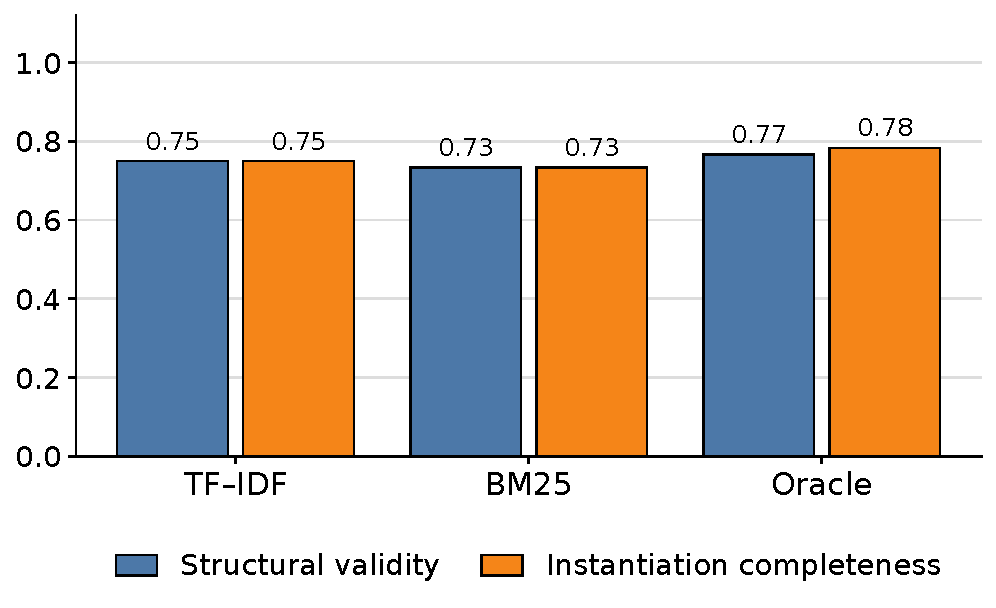
\includegraphics[width=0.75\linewidth]{figures/figure3_engineering_validation_comparison.pdf}
  \caption{Structural-validity and instantiation-completeness rates on the 60-instance subset, for TF--IDF, BM25, and Oracle schema retrieval.}
  \label{fig:eng-validation}
\end{figure}

\paragraph{Executable-attempt subset (269 instances).} Table~\ref{tab:eng-executable} reports the largest deterministic subset with non-empty gold \texttt{optimus\_code} (269 instances). Structural-validity and instantiation-completeness rates remain broadly consistent with the main benchmark (TF--IDF: $0.8141$ structural valid, $0.6654$ instantiation complete), but the executable, solver-success, feasible, and objective-produced rates are all $0.0$ for every baseline. The uniform blocker is a missing \texttt{gurobipy} runtime dependency (\texttt{ModuleNotFoundError}) in the evaluation environment used for this subset. We report this as a blocker study documenting an environment limitation, not as evidence that the retrieval-assisted grounding method itself produces zero executable value; the final solver-backed subset below shows nonzero outcomes once this dependency is removed by using a SciPy-based shim instead.

\begin{table}[t]
\centering
\caption{Executable-attempt subset (269 instances): schema-hit, structural-validity, and instantiation-completeness rates. The executable, solver-success, feasible, and objective-produced rates are uniformly $0.0$ for every baseline because of a missing \texttt{gurobipy} runtime in this evaluation environment (see text); they are omitted from the table as an environment blocker rather than a scientific result.}
\label{tab:eng-executable}
\small
\begin{tabular}{lccc}
  \toprule
  Baseline & Schema Hit & Structural Valid & Inst.\ Complete \\
  \midrule
  TF--IDF & 0.9368 & 0.8141 & 0.6654 \\
  BM25    & 0.9257 & 0.8104 & 0.6580 \\
  Oracle  & 1.0000 & 0.8253 & 0.6840 \\
  \bottomrule
\end{tabular}
\end{table}

\paragraph{Final solver-backed subset (20 instances).} To obtain a real, non-placeholder solver signal, we further filter to a 20-instance subset selected deterministically by a static shim-compatibility rule (non-empty gold \texttt{optimus\_code} and predicted code compatible with the SciPy HiGHS shim), capped at 20 instances. Table~\ref{tab:eng-solver} and Figure~\ref{fig:eng-solver} report executable, solver-success, feasible, and objective-produced rates for TF--IDF and Oracle retrieval. TF--IDF reaches $0.95$ executable, $0.80$ solver-success, $0.80$ feasible, and $0.80$ objective-produced; Oracle reaches $0.95$, $0.75$, $0.75$, and $0.75$, respectively. The non-executable rows in each baseline fail due to an indexing incompatibility in the shim path (\texttt{IndexError}), affecting 2 of 40 baseline-instance rows across the two baselines. Because this subset is small and selected by compatibility filtering rather than random sampling, these rates should be read as a restricted, pragmatic demonstration that the recovered structure can drive a real solver on compatible cases -- not as a benchmark-wide solver-readiness claim.

\begin{table}[t]
\centering
\caption{Final solver-backed subset (20 instances, SciPy HiGHS MILP compatibility shim; Gurobi not required).}
\label{tab:eng-solver}
\small
\begin{tabular}{lcccc}
  \toprule
  Baseline & Executable & Solver Success & Feasible & Objective Produced \\
  \midrule
  TF--IDF & 0.95 & 0.80 & 0.80 & 0.80 \\
  Oracle  & 0.95 & 0.75 & 0.75 & 0.75 \\
  \bottomrule
\end{tabular}
\end{table}

\begin{figure}[t]
  \centering
  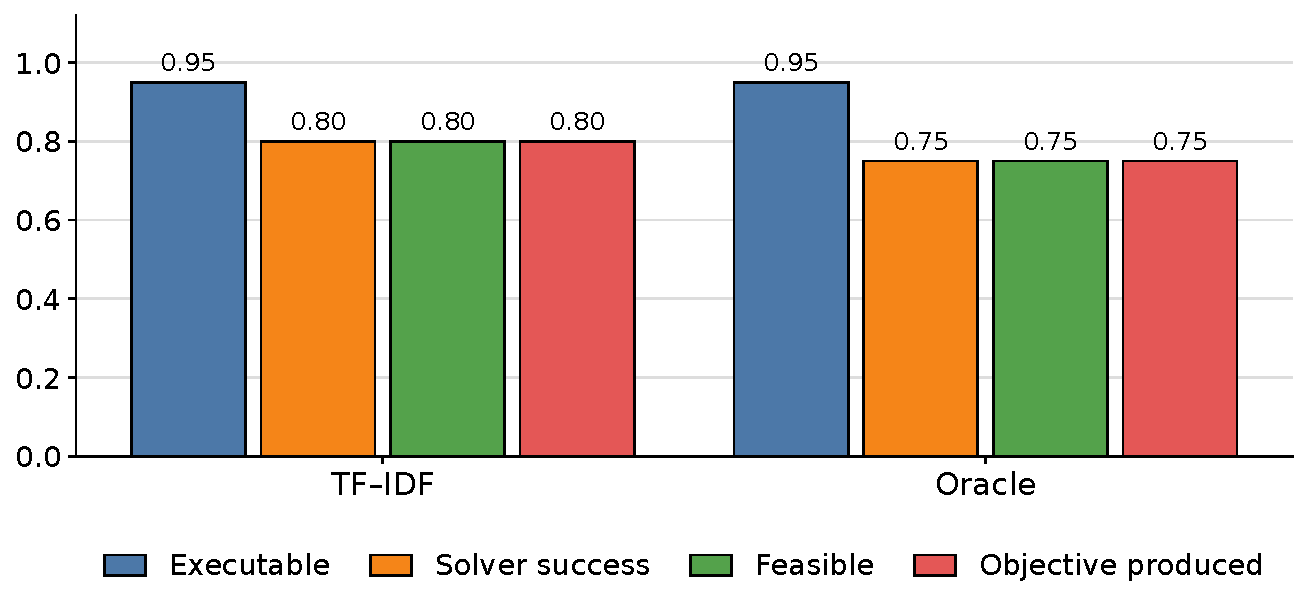
\includegraphics[width=0.75\linewidth]{figures/figure4_final_solver_backed_subset.pdf}
  \caption{Executable, solver-success, feasible, and objective-produced rates on the 20-instance final solver-backed subset (SciPy HiGHS shim), for TF--IDF and Oracle schema retrieval.}
  \label{fig:eng-solver}
\end{figure}

\paragraph{Summary.} Across all three validation studies, the same qualitative pattern from the main benchmark repeats: Oracle retrieval does not consistently provide a substantial advantage over TF--IDF, and the dominant limitation is downstream. On the structural subset Oracle is modestly higher than TF--IDF ($0.7667$ vs.\ $0.75$ structural-valid; $0.7833$ vs.\ $0.75$ instantiation-complete), but on the final solver-backed subset Oracle is actually \emph{lower} than TF--IDF on solver-success, feasible, and objective-produced rates ($0.75$ vs.\ $0.80$ on each), a difference plausibly attributable to this subset's small size (20 instances) and its compatibility-filtering rule rather than to a genuine retrieval-quality effect. Taken together, these restricted studies reinforce the main benchmark's conclusion that downstream grounding -- not schema selection -- is the binding constraint, and they caution against assuming a monotonic Oracle advantage on small subsets. In the executable-attempt subset, missing scalar slots, type mismatch, and incomplete instantiation account for the majority of non-\texttt{gurobipy} failures (69, 82, and 267 counted instances, respectively, across baselines), consistent with the error taxonomy in Section~\ref{subsec:exp_error}. These restricted studies should be read as evidence of downstream engineering relevance on compatible cases, complementing -- not replacing -- the main scalar-grounding benchmark.

\section{Conclusions and Future Research}
\label{sec:conclusion}

This paper studied a retrieval-assisted approach to optimization problem instantiation from natural-language descriptions. Rather than targeting full solver-ready generation, we focused on a narrower intermediate task: retrieving a compatible optimization schema from a fixed catalog and then instantiating its scalar parameters through deterministic grounding of numeric mentions in the query. This formulation isolates an important intermediate capability in natural-language-to-optimization pipelines: before full model synthesis can be attempted, the system must identify a plausible template and recover at least part of the quantitative information needed to instantiate it.

The main benchmark results lead to a clear conclusion. On the \textsc{NLP4LP} benchmark, schema retrieval is already strong for this task setting: BM25, TF--IDF, and LSA all substantially outperform random selection across the evaluated query variants, with TF--IDF again providing the strongest average top-1 retrieval performance. Thus, within this fixed-catalog benchmark, schema retrieval is not the dominant empirical bottleneck.

The main remaining challenge lies downstream. The benchmark shows that deterministic retrieval-assisted grounding can recover a substantial fraction of usable scalar structure on the original queries, and the strongest frozen non-oracle method, \texttt{tfidf\_typed\_greedy}, achieves \textit{InstantiationReady} $=0.8006$ (and \textit{StrictInstantiationReady} $=0.7704$) on the 331-query test split. However, the oracle result reaches only $0.8489$, so perfect schema selection yields only a modest additional gain over the strongest retrieval-based setting. This indicates that the dominant source of residual error is not selecting the broad problem type, but assigning extracted numeric mentions to the correct scalar roles once a plausible schema has been retrieved. In other words, the main bottleneck in the current pipeline is number-to-slot grounding under semantic ambiguity.

At the same time, the frozen numeric-extraction ablation shows that correcting how ratio-word quantities are extracted produces meaningful gains in \textit{TypeMatch}, \textit{InstantiationReady}, and \textit{StrictInstantiationReady} while leaving retrieval-dependent quantities unchanged. Together with the error taxonomy, these findings indicate that the remaining difficulty is not simply a lack of downstream engineering variety, but a more fundamental challenge of semantically determining which quantity in the query plays which optimization role.

Beyond the core benchmark, the structural and solver-backed validation studies in Section~\ref{subsec:exp_engineering} give a more practical perspective. TF--IDF and Oracle retrieval produce structurally valid, instantiation-complete artifacts on $75$--$78\%$ of the 60-instance structural subset (Table~\ref{tab:eng-structural}); the 269-instance executable-attempt subset documents a transparent environment blocker (a missing \texttt{gurobipy} runtime) rather than a property of the method (Table~\ref{tab:eng-executable}); and on the 20-instance final solver-backed subset, TF--IDF reaches $0.80$ solver-success, feasible, and objective-produced rates versus $0.75$ for Oracle (Table~\ref{tab:eng-solver}) -- Oracle is not consistently better across the three studies, again underscoring that downstream grounding, not schema selection, is the binding constraint. These subsets are intentionally narrow and should not be read as benchmark-wide solver readiness, but they show the recovered structure can drive a real solver on compatible cases.

The contribution of the paper should therefore be understood in a measured way: not a complete natural-language-to-optimization compiler, nor a replacement for an optimization modeler, but a transparent retrieval-and-instantiation component with measurable downstream value for intelligent decision support, in the sense already discussed in Section~\ref{subsec:intro_contributions}.

It is worth stating explicitly what the inference-time LLM-free property does and does not imply. The proposed method requires no large language model at inference time: schema retrieval and scalar parameter grounding are fully deterministic and CPU-only, which makes every intermediate decision inspectable, reproducible, and independent of paid API access or dedicated GPU compute. This is a meaningful operational property for decision-support workflows that require auditability and deterministic behavior. It is not, however, evidence that deterministic lexical retrieval and rule-based grounding are generally superior to LLM-based modeling. End-to-end LLM systems target a broader, open-ended synthesis task -- producing complete formulations and solver code from text -- that the present fixed-catalog scalar-instantiation setting deliberately does not attempt. The two families sit on different points of a cost--capability tradeoff, and the preliminary external-baseline assessment in Section~\ref{subsec:exp_external} is presented precisely to make that tradeoff visible rather than to rank systems. Within its scope, the present study shows what can be achieved without generative inference, while leaving open the possibility that hybrid systems -- transparent schema retrieval paired with stronger learned or LLM-based downstream grounding (Section~\ref{subsec:future_work}) -- are a promising direction.

\subsection{Limitations and Threats to Validity}
\label{subsec:limitations}

The scope restrictions adopted throughout this paper (Section~\ref{subsec:method_problem}) are deliberate design choices, but they also bound what the results can and cannot support. We summarize the main limitations and threats to validity here rather than leaving them dispersed across the paper.

\emph{Fixed-catalog retrieval.} Schema retrieval is evaluated only as a 335-way identification problem over the benchmark-induced catalog described in Section~\ref{subsec:method_retrieval}. The strong retrieval numbers in Section~\ref{subsec:exp_retrieval} characterize this fixed-catalog setting and should not be read as evidence that lexical retrieval would remain competitive against an open-domain or substantially larger schema library, where semantic rather than lexical retrieval may become necessary.

\emph{Dataset dependence and lexical overlap.} All quantitative results are computed on \textsc{NLP4LP}, a single benchmark. The overlap-based stress tests in Section~\ref{subsec:exp_significance} show that retrieval accuracy is not simply an artifact of numeric-value overlap between query and schema text, but the diagnostic medium-overlap bucket contains only 4 of 331 \emph{orig} queries -- too few to fully rule out benchmark-specific lexical or structural regularities at scale. Generalization to optimization problem descriptions written in different styles, domains, or languages is untested.

\emph{Gated data access.} \textsc{NLP4LP} requires an approved Hugging Face account and access token (Declarations, Data availability). Independent researchers can inspect and rerun analyses on the committed result artifacts without this access, but a full end-to-end rerun on live benchmark queries requires it, which is a real (if benchmark-typical) reproducibility constraint.

\emph{Scalar-only instantiation.} The benchmarked instantiation stage recovers only scalar parameters; list-valued, vector-valued, and dictionary-valued parameters are out of scope (Section~\ref{subsec:method_design}). The reported \textit{Coverage}, \textit{TypeMatch}, and \textit{InstantiationReady} scores therefore characterize a restricted parameter-recovery problem, not full model-parameter reconstruction.

\emph{Heuristic type and role inference.} Both coarse type inference (Section~\ref{subsec:method_instantiation}) and optimization-role compatibility (Section~\ref{subsec:method_instantiation}) are deterministic, lexicon- and rule-based mechanisms with no formal correctness guarantee. The error taxonomy (Table~\ref{tab:nlp4lp-error-taxonomy}) indicates that this heuristic layer is also the paper's main open problem: semantic quantity-to-role ambiguity is not resolved by the methods evaluated here.

\emph{Restricted and small solver-backed validation.} The structural and solver-backed studies in Section~\ref{subsec:exp_engineering} use restricted subsets (60, 269, and 20 instances, respectively) selected by data-availability or compatibility filtering rather than random sampling, and the only solver evaluated is SciPy's open-source HiGHS backend; Gurobi and other commercial or specialized solvers are not exercised. The 20-instance final solver-backed subset in particular is too small to support benchmark-wide solver-readiness claims, and the 269-instance executable-attempt subset reports a uniform environment blocker (a missing \texttt{gurobipy} runtime) rather than a fully executed solver comparison.

\emph{Limited direct comparison against end-to-end LLM systems.} Section~\ref{sec:related_work} discusses several recent end-to-end large-language-model-based optimization-modeling systems (e.g., OptiMUS, OptLLM, Chain-of-Experts, LLMOPT, OPT2CODE, ORLM, OptMATH) qualitatively, and the repository documents a preliminary external-baseline assessment on a small common-18 subset in which PaMOP and OptMATH complete (18/18 and 15--18/18 on available solver runs) and a generic LLM completes 16/18, while ORLM's released checkpoint could not be executed because its solver dependency (\texttt{coptpy}) is unavailable and DeepOR/OR-R1 do not release official checkpoints. However, this paper does not run these systems head-to-head against the proposed pipeline on the full \textsc{NLP4LP} benchmark. These systems target a different, broader task (full formulation and solver-code generation) and typically depend on paid API access or substantial compute, which was outside the scope and budget of this study; a controlled quantitative comparison is left to future work.

\emph{No external dataset validation or deployment study.} Although Section~\ref{sec:related_work} discusses \textsc{Text2Zinc} and \textsc{CP-Bench} as related benchmarks, the framework is not evaluated on them or on any other external dataset in this paper, so cross-benchmark generalization is untested. Similarly, no user study or production deployment was conducted; the practical-usefulness claims in this paper are limited to the restricted, benchmark-scoped, and subset-based evidence reported in Sections~\ref{subsec:exp_downstream}--\ref{subsec:exp_engineering}.

\subsection{Future Research Directions}
\label{subsec:future_work}

Several directions for future research follow naturally from these findings. The first is to strengthen the downstream grounding stage itself with substantially stronger semantic role-sensitive methods, rather than additional variants of the current deterministic assignment family. The second is to extend the current scalar-only setting to more structured parameter types, including vectors, indexed collections, and dictionary-valued arguments. The third is to explore hybrid systems in which transparent schema retrieval provides structural scaffolding for stronger learned or large-language-model-based downstream grounding modules. A fourth direction is to expand the current restricted engineering validations into broader executable studies with more complete solver-backed coverage and wider template support.

More broadly, the results suggest that intermediate capabilities such as schema retrieval, schema-conditioned slot selection, and partial structured instantiation deserve independent attention in the design of transparent optimization support systems. Full natural-language-to-optimization automation remains difficult, but intermediate systems can already provide useful support by narrowing candidate problem structure and recovering part of the quantitative content needed for formal modeling. At the same time, the present results make clear that robust quantity-to-role grounding remains unresolved even when retrieval is strong. This makes the intermediate task studied here both practically relevant and scientifically valuable as a benchmarked subproblem in natural-language-to-optimization research.

\section*{Acknowledgements}

The author is deeply grateful to his mother for her continuous emotional support. The author also thanks his PhD advisor, Professor Ioannis Koutis, for his support, guidance, and encouragement, and Anders Borum for generously providing complimentary lifetime access to Secure ShellFish, which supported the author's remote research workflow.

\section*{Declarations}

\noindent\textbf{Funding.} This research did not receive any specific grant from funding agencies in the public, commercial, or not-for-profit sectors. The external large-language-model baselines reported in Section~\ref{subsec:exp_external} were executed through Microsoft Azure OpenAI API access; no other cloud-computing or API resources contributed to the experiments reported in this paper.
% TODO(AUTHOR_CONFIRMATION_REQUIRED): confirm that the Microsoft Azure for Students
% subscription credit (USD 100, valid approximately one year) is the funding source
% of the Azure OpenAI calls used for the external baselines in Section
% \ref{subsec:exp_external}, and that the disclosure sentence above is accurate;
% otherwise rephrase. Google Cloud Research Credits, the Cohere Catalyst Grant, and
% Fireworks/AMD credits are intentionally NOT acknowledged because they did not
% demonstrably contribute to this paper's reported computation, and the external
% LLM baselines are scientific comparison systems, not manuscript-preparation
% assistance (which is disclosed separately below).

\noindent\textbf{Competing interests.} The author declares that there are no known competing financial interests or personal relationships that could have appeared to influence the work reported in this paper.

\noindent\textbf{Ethics approval.} Not applicable; this study did not involve human participants, human data, or animals.

\noindent\textbf{Author contributions (CRediT).} Soroush Vahidi: Conceptualization, Methodology, Software, Validation, Formal analysis, Investigation, Data curation, Writing -- original draft, Writing -- review \& editing, Visualization. This single-author paper uses the standard CRediT taxonomy to describe the contributions of the sole author.

\noindent\textbf{Data availability.} The benchmark used in this paper, NLP4LP (\texttt{udell-lab/NLP4LP} on Hugging Face), is a gated third-party dataset that requires an approved Hugging Face account and access token; it is not redistributed by the author. The committed frozen result artifacts, camera-ready tables, figures, and analysis reports summarizing results computed from this dataset are available at \url{https://github.com/SoroushVahidi/combinatorial-opt-agent} (see \texttt{results/} and \texttt{analysis/}). This corresponds to Elsevier's Data availability Option C (data shared on request / availability statement with a repository link).

\noindent\textbf{Code availability.} The retrieval, grounding, evaluation, and figure/table-generation code used in this paper is available at \url{https://github.com/SoroushVahidi/combinatorial-opt-agent}. Reading the committed tables and figures, and running the test suite, do not require Hugging Face dataset access; reproducing a full end-to-end rerun on NLP4LP (retrieval and grounding on the live benchmark) requires the gated dataset access described above.

\section*{Declaration of generative AI and AI-assisted technologies in the manuscript preparation process}

During the preparation of this work the author used ChatGPT and Gemini to assist with aspects of manuscript writing and Cursor and GitHub Copilot to assist with coding. After using these tools/services, the author reviewed and edited the content as needed and takes full responsibility for the content of the published article. This declaration concerns manuscript preparation only; the scientific method evaluated in this paper requires no large language model at inference time, and the large-language-model systems discussed in Sections~\ref{sec:related_work} and~\ref{subsec:exp_external} are external comparison systems, not manuscript-preparation assistance.

\bibliographystyle{elsarticle-num}
\bibliography{references}

\end{document}